%----------------------------------------------------------------------------------------
% DOCUMENT SPECIFICATION
%----------------------------------------------------------------------------------------
\documentclass[
    11pt,                      % Default font size
    %oneside,                  % One-side binding. Default: Two-side binding / alternating margins
    english,                   % Language. Use ngerman for German (Neue Rechtschreibung)
    singlespacing,             % Spacing option: singlespacing, onehalfspacing or doublespacing
    %nolistspacing,            % Set spacing in lists to single
    %draft,                    % Enable draft mode: no pictures, no links, overfull hboxes indicated
    liststotoc,               % Include list of figures/tables/etc in the table of contents
    %toctotoc,                 % Include the main table of contents to the table of contents
    parskip,                  % Add vertical space between paragraphs
    %nohyperref,               % Disable links in the entire document
    % helveticafont,             % Uncomment to use Helvetica font
    headsepline,               % Show a horizontal line under the header
    %chapterinoneline,         % Place the chapter title and chapter number on one line
    consistentlayout,          % Have the same layout for special chapters: declaration, abstract and acknowledgements
]{MastersDoctoralThesis}

% Uncomment the following lines to only include a subset of chapters.
% This is useful for long documents, as typesetting takes a bit of time
%\includeonly{
%    Front/titlepage,
%    Front/imprint,
%    Front/abstract,
%    %Front/declaration,
%    %Front/acknowledgements,
%    %Front/symbols,
%    Chapters/Chapter1,
%    %Chapters/Chapter2
%    }


%----------------------------------------------------------------------------------------
% PREAMBLE: PACKAGES AND CONFIGURATIONS
%----------------------------------------------------------------------------------------
\input{preamble}


%----------------------------------------------------------------------------------------
% THESIS INFORMATION: MODIFY THIS SECTION!
%----------------------------------------------------------------------------------------

\thesistitle{CorpusAgent - A Hybrid NLP and LLM-Based System for Large Text Corpus Analysis}             % Thesis title,              command: \ttitle
\thesistype{Project Thesis}             % Type of thesis (e.g. Master Thesis) \ttype
\thesisdate{\today}                     % Date of submission                  \tdate
\keywords{natural language processing}
                                        % Keywords for the thesis,            \keywordnames
\author{Moritz Feuchter\\Shpetim Veseli}                  % Your name,                          \authorname
\degree{Bachelor of Science ZHAW}          % Degree name,                        \degreename
\studyprogram{Computer Science} 
                                        % Study program                       \studyprog
\studyprogramlink{https://www.zhaw.ch/de/engineering/studium/bachelorstudium/informatik}
                                        % Link to study program               \studyproglink

\supervisorA{Prof. Dr. Mark Cieliebak}       % Name of supervisor 1,          \supnameA
\supervisorAmail{mark.cieliebak@zhaw.ch}         % Email address of supervisor 1,      \supmailA
\supervisorAinfo{                       % Formatted info about supervisor 1:  \supinfoA
    \supnameA\\
    Zurich University of Applied Sciences\\
    Email: \href{mailto:\supmailA}{\supmailA}\\
}

% Keep empty if there is no supervisor 2: \supervisorB{}
\supervisorB{Manuela Hürlimann}              % Name of supervisor 2,               \supnameB
\supervisorBmail{manuela.huerlimann@zhaw.ch}       % Email address of supervisor 2,      \supmailB
\supervisorBinfo{                       % Formatted info about supervisor 2:  \supinfoB
    \supnameB\\
    Zurich University of Applied Sciences\\
    Email: \href{mailto:\supmailB}{\supmailB}\\
}

\university{Zurich University of Applied Sciences}
                                        % University name                     \univname
\universitygerman{Zürcher Hochschule für Angewandte Wissenschaften}
                                        % University, in German               \univnameger
\unversityabbr{ZHAW}                    % University abbreviation             \univabbr

\department{School of Engineering} 
                                        % Department,                         \deptname
% \institute{} 
                                        % Institute,                          \instname
% \group{Center of Computational Health} 
                                        % Research group                      \groupname

% Links
\universitylink      {https://www.zhaw.ch/en/university/}                   % \univlink
\universitylinkgerman{https://www.zhaw.ch/de/university/}                   % \univlinkger
\departmentlink      {https://www.zhaw.ch/en/engineering}                         % \deptlink
% \institutelink       {} % \instlink
% \grouplink           {} % \grplink



\AtBeginDocument{
\hypersetup{pdftitle=\ttitle} % Set the PDF's title to your title
\hypersetup{pdfauthor=\authorname} % Set the PDF's author to your name
\hypersetup{pdfkeywords=\keywordnames} % Set the PDF's keywords to your keywords
}

\begin{document}
\frontmatter                  % Roman page numbering for the pre-content pages
\pagestyle{plain}             % Default to the plain heading style until the thesis style 
                              % is called for the body content


%----------------------------------------------------------------------------------------
% TITLE PAGE AND IMPRINT
%----------------------------------------------------------------------------------------
\include{Front/titlepage}
\let\cleardoublepage\clearpage
\include{Front/imprint}


%----------------------------------------------------------------------------------------
% DECLARATION
%----------------------------------------------------------------------------------------
% Comment out this section if the declaration of originality from ZHAW is used.
% \include{Front/declaration}
% \cleardoublepage


%----------------------------------------------------------------------------------------
% ABSTRACT
%----------------------------------------------------------------------------------------
% !TEX root = ../main.tex

%----------------------------------------------------------------------------------------
% ABSTRACT PAGE
%----------------------------------------------------------------------------------------
\begin{abstract}
\addchaptertocentry{\abstractname} % Add the abstract to the table of contents
Large news corpora provide rich information about real-world events and their public perception over time.\\
However, extracting meaningful insights from such corpora is challenging due to their size, temporal complexity, and the fragmented nature of relevant information. Classical natural language processing techniques enable scalable extraction of structured signals but require substantial manual interpretation, while large language models offer high-level reasoning but cannot directly process large document collections.

This thesis presents CorpusAgent, a hybrid analysis system designed for exploratory analysis of large news corpora. The system combines classical NLP methods for scalable signal extraction with LLM-based reasoning for planning, synthesis, and explanation. A database-centric architecture is used to store documents and intermediate results, enabling reproducible analyses and traceable answers to complex, temporally structured research questions.

The approach is evaluated through a set of longitudinal case studies on a large English-language news corpus, covering topics such as political coverage, corporate crises, public health events, and social movements. The results demonstrate that CorpusAgent can autonomously decompose complex analytical questions, select appropriate analytical NLP tools, and synthesize coherent, context-aware interpretations while explicitly handling uncertainty, missing evidence, and false premises. \\
This work contributes a system-level perspective on how LLMs can be integrated responsibly into large-scale text analysis workflows, focusing on analytical reliability, interpretability, and exploratory use rather than the development of new NLP models.
\end{abstract}


%----------------------------------------------------------------------------------------
% ACKNOWLEDGEMENTS
%----------------------------------------------------------------------------------------
% !TEX root = ../main.tex

%----------------------------------------------------------------------------------------
% ACKNOWLEDGEMENTS
%----------------------------------------------------------------------------------------
\begin{acknowledgements}
\addchaptertocentry{\acknowledgementname} % Add the acknowledgements to the table of contents

I would like to thank my supervisors, Prof. Dr. Mark Cieliebak and Manuela Hürlimann, for their guidance, valuable feedback, and support throughout this thesis.

I also thank my project partner for the constructive collaboration, technical discussions, and shared effort in the design and implementation of the CorpusAgent system.

Finally, I am grateful to my family and friends for their support during my studies.
\end{acknowledgements}



%----------------------------------------------------------------------------------------
% LIST OF CONTENTS/FIGURES/TABLES PAGES
%----------------------------------------------------------------------------------------
% Comment out if any of the following is not needed:
\tableofcontents  % Add main table of contents
%\listoffigures    % Add list of figures
%\listoftables     % Add list of tables


%----------------------------------------------------------------------------------------
% ABBREVIATIONS / SYMBOLS
%----------------------------------------------------------------------------------------
% !TEX root = ../main.tex

%----------------------------------------------------------------------------------------
% ABBREVIATIONS
%----------------------------------------------------------------------------------------

% List of abbreviations: a table of two columns.
\begin{abbreviations}{ll}

\textbf{IR} & \textbf{I}nformation \textbf{R}etrieval\\
\textbf{LLM} & \textbf{L}arge \textbf{L}anguage \textbf{M}odel\\
\textbf{RAG} & \textbf{R}etrieval-\textbf{A}ugmented \textbf{G}eneration\\
\textbf{NLP} & \textbf{N}atural \textbf{L}anguage \textbf{P}rocessing\\
\textbf{API}   & \textbf{A}pplication \textbf{P}rogramming \textbf{I}nterface\\
\textbf{AWS}   & \textbf{A}mazon \textbf{W}eb \textbf{S}ervices\\
\textbf{BTC}   & \textbf{B}it\textbf{c}oin\\
\textbf{EV}    & \textbf{E}lectric \textbf{V}ehicle\\
\textbf{JSON}  & \textbf{J}ava\textbf{S}cript \textbf{O}bject \textbf{N}otation\\
\textbf{JSONB} & \textbf{J}ava\textbf{S}cript \textbf{O}bject \textbf{N}otation \textbf{B}inary (PostgreSQL specific)\\
\textbf{LDA}   & \textbf{L}atent \textbf{D}irichlet \textbf{A}llocation\\
\textbf{RDBMS} & \textbf{R}elational \textbf{D}atabase \textbf{M}anagement \textbf{S}ystem\\
\textbf{SQL}   & \textbf{S}tructured \textbf{Q}uery \textbf{L}anguage\\
\textbf{UI}    & \textbf{U}ser \textbf{I}nterface\\
\textbf{VIX}   & \textbf{V}olatility \textbf{I}nde\textbf{x} (CBOE)\\

\end{abbreviations}


%----------------------------------------------------------------------------------------
% PHYSICAL CONSTANTS/OTHER DEFINITIONS
%----------------------------------------------------------------------------------------

%% List of physical constants: a three column table
%\begin{constants}{lr@{${}={}$}l} 
%
%% The \SI{}{} command is provided by the siunitx package, see its documentation 
%% for instructions on how to use it
%
%Speed of Light & $c_{0}$ & \SI{2.99792458e8}{\meter\per\second} (exact)\\
%%Constant Name & $Symbol$ & $Constant Value$ with units\\
%
%\end{constants}


%----------------------------------------------------------------------------------------
% SYMBOLS
%----------------------------------------------------------------------------------------

%% List of Symbols: a three column table
%\begin{symbols}{lll} 
%
%$a$ & distance & \si{\meter} \\
%$P$ & power & \si{\watt} (\si{\joule\per\second}) \\
%%Symbol & Name & Unit \\
%
%\addlinespace % Gap to separate the Roman symbols from the Greek
%
%$\omega$ & angular frequency & \si{\radian} \\
%
%\end{symbols}



%----------------------------------------------------------------------------------------
% DEDICATION
%----------------------------------------------------------------------------------------
% \dedicatory{For/Dedicated to/To my\ldots} 


%----------------------------------------------------------------------------------------
% THESIS CONTENT - CHAPTERS
%----------------------------------------------------------------------------------------
\mainmatter % Begin numeric (1,2,3...) page numbering
\pagestyle{thesis} % Return the page headers back to the "thesis" style


% Include the chapters of the thesis as separate files from the Chapters folder
% Uncomment the lines as you write the chapters

% !TEX root = ../main.tex
%----------------------------------------------------------------------------------------

% INTRODUCTION CHAPTER

\chapter{Introduction} % Main chapter title

\label{Chapter1}

Large news corpora contain detailed records of real-world events and their public perception over time. They document how topics emerge, how narratives evolve, and how different actors are portrayed across sources and time periods.

Such data offers significant potential for research in areas such as media analysis, economics, and political science.
At the same time, extracting meaningful insights from large news corpora is difficult. Relevant information is distributed across many documents, sources, and time spans, making manual analysis impractical or even impossible. \\
Many research questions are inherently complex and temporal, for example how media sentiment changes during a corporate crisis or how thematic focus shifts throughout major events. Simple keyword searches or document-level summaries are not powerful enough to answer such questions.
Classical natural language processing techniques enable scalable extraction of structured signals such as entities, keywords, sentiment, and topics. However, these methods typically produce results that require substantial manual interpretation since they lack deep reasoning capabilities.

Recent Large Language Models, on the other hand, can generate coherent natural-language explanations but cannot reliably operate directly on large corpora because of input size limitations (e.g. context windows) and high computational costs.
This tension reveals a gap between scalable corpus-level analysis and high-level, interpretable reasoning.
This thesis addresses this gap by presenting a hybrid analysis system for large news corpora. The proposed approach combines classical NLP methods for scalable, structured analysis with LLM-based reasoning for synthesis and explanation. A database-centric architecture is used to store documents and intermediate results, enabling reproducible analyses and traceable answers to complex research questions.
The objective of this project is to demonstrate how such a system can support large-level analysis of big data collections. The approach is evaluated using case studies on a large English-language news corpus, showing how temporal developments, sentiment shifts, and thematic changes can be analyzed and explained in an integrated manner.

This thesis focuses on system design and applied analysis rather than the development of new NLP models. Its contribution lies in the integration of existing methods into a coherent architecture and in demonstrating how LLMs can be used responsibly and effectively as part of a larger analytical workflow.

% Indicate the main file. Must go at the beginning of the file.
% !TEX root = ../main.tex

%----------------------------------------------------------------------------------------
% CHAPTER TECHNICAL BACKGROUND
%----------------------------------------------------------------------------------------

\chapter{Technical Background}
\label{ChapterTechnicalBackground}

%----------------------------------------------------------------------------------------

\section{Challenges in Large-Scale Text Corpus Analysis}

Large-scale text corpora, such as news archives, web crawls, or social media collections, have become indispensable sources for understanding social discourse, public perception, and temporal dynamics across domains. Their volume, however, lead non-trivial methodological and technical challenges for extraction of high-level insights.

\subsection{Scala and Volume}

The size of contemporary textual corpora can render traditional manual or small-scale qualitative approaches infeasible. In studies of social media or news media, researchers have noted that large corpora both enable and constrain analysis, as simple text retrieval and manual content inspection become impractical without automated processing pipelines \cite{moreno2023strategies}. Computational infrastructure and scalable indexing are required to manage terabytes of raw text and to support iterative exploratory workflows.

\subsection{Fragmentation Across Sources and Time}

Unlike carefully curated datasets, real-world corpora are often heterogeneous in source, format, and temporal coverage. This fragmentation complicates cross-source and longitudinal analyses, where differences in publication norms, metadata standards, or archive completeness can bias results unless explicitly addressed. Fragmentation also increases the complexity of defining consistent temporal units (e.g., weeks, months, phases) across different collections.

\subsection{Temporal and Comparative Analysis Challenges}

Understanding how narratives evolve over time (for example, how sentiment or topic distributions shift across years or in response to events) demands methods that can extract macroscopic patterns from massive text sequences \cite{lansdall2018history}. Classical retrieval or simple keyword counts might indicate presence or absence of terms, but temporal dynamics requires scalable trend detection and segmentation algorithms that can operate over millions of documents and across long time spans. Simple frequency analysis may misrepresent underlying shifts due to seasonality or publication rate variations.

\subsection{Limits of Manual Qualitative Analysis}

Traditional content and discourse analysis in fields such as journalism relies heavily on human interpretation of text. When your corpora scale gets beyond a few thousands documents, such manual techniques become prohibitively time-consuming and prone to inconsistency. This underscores the need for computational methods that can provide reproducible, scalable, and interpretable summaries and metrics without replacing human insight entirely.

%----------------------------------------------------------------------------------------

\section{Classical Information Retrieval and Text Analysis Pipelines}

Before the rise of large language models and neural reasoning systems, classical information retrieval (IR) and text analysis were the core methods for extracting relevant information from large text corpora. These systems are optimized for scalable keyword matching and ranking, but they fundamentally lack mechanisms for higher-level synthesis or narrative reasoning.

At the core of most classical IR systems is the inverted index, a data structure that maps terms to the documents in which they appear. An inverted index enables efficient lookup of documents containing particular keywords, and it forms the backbone of virtually all large-scale search systems and full-text search engines \cite{ir_inverted_index}. By precomputing term-to-document mappings, inverted indices allow queries to be answered in time proportional to the number of matching documents rather than the size of the entire corpus.

Traditional IR systems differ from generic relational database (RDB) text search in both structure and performance. While many RDBMS support text search through full-text indices or simple keyword matching functions, they do not implement inverted indices with optimized postings lists and ranking functions, and they typically scale poorly as corpus size increases. Search engines and dedicated IR libraries implement query processing, ranking, and caching strategies that deliver both higher precision and better performance on large document collections.

These classical approaches have several operational strengths. Because they rely on well-understood algorithms and data structures, they offer predictable scalability to millions or billions of documents, reproducible results under identical query setups, and transparent ranking heuristics that can be interpreted or tuned by system designers. They support keyword matching and partial boolean logic constructs that make them suitable for applications where exact text occurrences are the primary retrieval signal.

At the same time, classical IR systems have important limitations. Keyword rankings mainly measure term overlap and rarity, so they do not produce narrative explanations or capture deeper meaning beyond surface words. These systems can return lists of likely documents, but they do not summarize results, compare trends, or reason about changes over time. They also miss relevant content when queries use different wording than the documents (vocabulary mismatch) unless combined with methods like query expansion or semantic re-ranking \cite{ir_retrieval_semantic}. For these reasons, IR alone is not sufficient as the final analytic layer for the complex, longitudinal questions addressed in this thesis.

%----------------------------------------------------------------------------------------

\section{Longitudinal and Temporal Analysis of News Corpora}

Analyzing how text changes over time is a central concern when working with large news corpora. This type of analysis is often referred to as diachronic analysis and involves studying patterns in language use, sentiment, topic prevalence, or framing across years, months, or other time intervals. In contrast to static or synchronic analysis, which examines text at a single point, diachronic approaches seek to uncover how content evolves and what that evolution might signify in terms of social, political, or cultural trends.

A diachronic corpus is defined as a collection of documents that are associated with timestamps spanning an extended period. Such corpora enable retrospective retrieval and temporal pattern study, as text from different time periods can be directly compared to identify trends in usage, topics, or sentiment \cite{ir_temporal_ir}. These temporal corpora are common in news analytics research, with examples ranging from multi-decade newspaper archives to structured headline collections used in sentiment dynamics studies \cite{10.1371/journal.pone.0276367}.

One important area of longitudinal analysis is understanding how narratives and frames change over time. In media and communication research, framing refers to the way information is presented and structured by news sources. Frame analysis has roots in social science and shows that the same issue can be described differently depending on context, emphasis, or intent, and that these representations shape audience interpretation \cite{frame_analysis_wikipedia}.

Another dimension of longitudinal analysis is topic or semantic shift detection. Over long time spans, not only do the topics covered by news outlets change, but the meanings of words and associations between concepts can shift. Computational methods for measuring such semantic change include diachronic word embeddings and time series models, which quantify how word contexts evolve in large corpora \cite{dukic2025characterizing}. These methods highlight that diachronic analysis can extend beyond simple counts and into deeper semantic dynamics.

Overall, longitudinal and temporal analysis of news corpora provides a systematic way to track change and compare narrative features across time. This type of analysis underlies many of the evaluation questions defined in this thesis, where changes in sentiment, topic distribution, or framing over years serve as the primary evidence for answering analytical queries.


%----------------------------------------------------------------------------------------
\section{Large Language Models}

Large Language Models (LLMs) are neural network–based systems trained on very large text corpora to perform language tasks such as generation, summarization, and reasoning over text. They are built on modern architectures that allow them to capture linguistic patterns and semantic relationships from vast datasets, making them powerful tools for natural language understanding and synthesis \cite{large_language_model_wikipedia}.

\subsection{Capabilities Relevant to This Thesis}

LLMs are particularly useful for synthesizing information across documents and producing coherent natural-language outputs based on structured inputs. For example, they can summarize long passages of text, identify central themes, and abstract key points from varied sources, supporting tasks such as literature review, topic interpretation, and summarization of complex content \cite{bigoulaeva2025inherent}\cite{what_are_llms_ibm}. In the context of this thesis, these capabilities enable the model to:
\begin{itemize}
    \item Transform structured analysis results (e.g., sentiment scores, topic distributions) into natural-language narratives.
    \item Integrate multi-stage analytic outputs into a unified answer that reads coherently and is easy for humans to interpret.
    \item Follow natural language instructions in prompts to guide how synthesis should proceed.
\end{itemize}

This makes LLMs valuable as a reasoning and explanation layer in an analytics pipeline: they go beyond keyword matching or quantitative metrics (like IR) to produce human-readable explanations of aggregated patterns.

\subsection{Limitations}

Despite their strengths, LLMs have known limitations that are important to consider in analytical systems. One fundamental constraint is the \textit{context window}: \\
LLMs can only process a limited number of tokens at once, making them unsuitable for analyzing large corpora directly without pre-processing or structured intermediate representations \cite{large_language_model_wikipedia}. Additionally, LLMs can produce outputs that appear plausible but are not grounded in the source data, a phenomenon known as \textit{hallucination}, especially in multi-document summarization tasks \cite{belem2025singlemultillmshallucinate}. These limitations mean that LLMs are best used in combination with structured retrieval and analysis components that provide them with relevant, condensed inputs rather than raw corpora.

By combining LLM capabilities with classical retrieval and analytic methods, a hybrid pipeline can leverage the strengths of both. Scalable preprocessing and indexing from classical approaches, and flexible synthesis and explanation from LLMs.

%----------------------------------------------------------------------------------------

\section{Retrieval-Augmented Generation and Related Architectures}

As large language models (LLMs) became practical for real-world use, researchers and practitioners developed hybrid approaches that combine retrieval mechanisms with some form of generation or reasoning. These tools aim to mitigate known limitations of standalone LLMs by grounding model outputs in external sources. Among these, Retrieval-Augmented Generation (RAG) has emerged as a prominent pattern, but it is not the only retrieval-based method in the landscape.

\subsection{Standard RAG Architecture}

Retrieval-Augmented Generation refers to architectural patterns in which a language model’s generation step is explicitly augmented with text retrieved from an external source at the time of query. Instead of relying solely on the model’s pretrained weights, RAG systems first retrieve relevant documents from a knowledge base or corpus, and then incorporate those texts as context for answer generation \cite{rag_wikipedia}\cite{what_is_rag_ibm}.  \\
This workflow typically consists of three high-level stages: (1) retrieval: locating relevant passages or documents, (2) augmentation: use these retrieved texts as additional conditioning context, and (3) generation: using the LLM to produce a response that combines retrieved evidence with the model’s own knowledge \cite{rag_wikipedia}.

The motivation behind RAG is to expand the knowledge available to the generative model without retraining it whenever new or domain-specific information becomes available. By indexing external sources and retrieving them at query time, RAG systems can produce outputs that are more accurate, up-to-date, and contextually grounded than generation based solely on pretrained parameters \cite{rag_openai}.

\subsection{Related Retrieval-Based Architectures}

Beyond RAG, several related architectures leverage retrieval to enhance language model capabilities. These include:
\begin{itemize}
    \item \textbf{Semantic Search:} Semantic search systems use vector-based retrieval to find documents that are semantically similar to a query, often using embeddings generated by LLMs themselves.
    \item \textbf{Hybrid Retrieval Systems:} These systems combine traditional keyword-based retrieval with semantic or embedding-based methods to improve recall and relevance.
    \item \textbf{Modular RAG Variants:} Some RAG implementations separate retrieval and generation more distinctly, allowing for different models or algorithms to be used at each stage, or incorporating multiple retrieval passes.
    \item \textbf{Orchestration Frameworks:} These frameworks manage complex workflows that involve multiple retrieval and generation steps, often integrating external tools or APIs to enhance reasoning capabilities.
\end{itemize}

\subsection{Strengths in Context}

These retrieval-enhanced models and tools share some common strengths:

\begin{itemize}
    \item By leveraging up-to-date external sources, they can produce outputs that are more accurate than relying on static model parameters \cite{what_is_rag_ibm}.
    \item They enable integration of domain-specific or proprietary content without retraining the LLM.
    \item Retrieval components can increase the chance that generated responses reference evidence relevant to the query.
\end{itemize}

\subsection{Limitations Relative to Corpus-Level Analysis}

Despite the advantages of retrieval-based approaches like Retrieval-Augmented Generation (RAG), these systems still have limitations that affect their usefulness for broad corpus analysis. RAG depends heavily on the quality and organisation of the external data it retrieves; if the underlying database contains outdated, irrelevant, or poorly indexed information, the retrieved context may be insufficient or misleading, and generated outputs can reflect these issues \cite{blog_rag_vs_buzz}. Even with retrieval, language models can still produce inaccurate or hallucinated responses if they misinterpret or overgeneralise from the retrieved text, because grounding does not guarantee correct interpretation \cite{rag_wikipedia}. \\
Furthermore, RAG systems are optimised to fetch a limited set of relevant documents per query rather than to summarise patterns across an entire corpus, which makes them less suitable for tasks that require aggregation over large document sets or comparison of trends over time. In addition, the retrieval process itself has challenges such as handling ambiguous queries.\cite{rag_problems_ibm}.

Because of these constraints, retrieval-enhanced architectures like RAG are effective for factually grounded, single-query tasks but are not designed to provide the structured, corpus-wide temporal reasoning required in the analyses pursued in this thesis.

%----------------------------------------------------------------------------------------

\section{Related Work and Research Prototypes}

There are a variety of tools and systems aimed at helping users explore, analyze, or visualize large text collections. These range from interactive news analytics dashboards to visual analytics systems for document sets, and from corpus exploration interfaces to research prototypes that combine visual and interactive components with natural language processing.

One example is interactive dashboards built for news sentiment analysis. These systems fetch articles through APIs, apply sentiment analysis models like VADER, and present time-series trends, topic distributions, and word-based visualizations through interactive graphs and charts \cite{sentiment_dashboard_ijcrt}. \\
Such dashboards are useful for exploring real-time or recent sentiment trends and for gaining a quick overview of important themes in a narrow topic area. However, these tools rarely support deep, multi-stage analytical workflows that combine scalable retrieval, advanced temporal aggregation, and narrative synthesis.

Another class of tools focuses on visual analytics for document collections beyond simple dashboards. Systems like VICTORIOUS offer modules to support sensemaking for scoping reviews: users upload a set of documents, and the system provides topic maps, clustering, and interactive views to assist classification and assessment \cite{victorious2025visual}.

While such tools advance exploratory interaction over document sets, they are generally designed for curated subsets of data rather than for large, unfiltered corpora spanning long time periods.

There are also open source tools developed for corpus linguistics and text exploration. Voyant Tools is a web-based application that offers simple frequency lists, distribution plots, and word pattern analysis for uploaded corpora, making it suitable for small- to medium-scale text exploration \cite{voyant_tools_wikipedia}. Similarly, R packages such as corporaexplorer provide interactive interfaces to browse and examine collections of text, but they require pre-prepared corpora and do not integrate large-scale retrieval or analytic pipelines \cite{corporaexplorer}. These tools are useful for linguistic studies or exploratory analysis, but they do not typically support structured temporal reasoning or hybrid LLM-assisted synthesis.

In the research literature, there are prototypes that combine visualization with deeper text analysis. For example, CARTOLABE is a web-based visualization framework for navigating large textual corpora through topic projections and interactive semantic maps, enabling users to explore patterns at multiple scales \cite{cartolabe2020web}. Tools like TextEssence support interactive comparative analysis of semantic changes between corpora using word embeddings, offering visual insights into shifts between document sets \cite{textessence2021tool}. \\
More recent work, such as VisPile, integrates LLMs and knowledge graphs into visual analytics systems that assist analysts in grouping documents and validating evidence interactively \cite{vispile2025visual}. These systems show how visualization and AI can help with complex analysis tasks, but they are often designed for specific research scenarios or require expert users, and they do not directly address longitudinal narrative synthesis over very large news corpora.

Beyond research prototypes, commercial or industry-oriented tools such as Pulsar provide social listening and audience intelligence, combining text analytics with trend detection and visual reporting across news and social media sources \cite{pulsar_wikipedia}. These platforms excel at real-time monitoring and broad narrative detection over multiple channels, but they are typically closed systems with limited transparency into intermediate analytic steps and without custom pipeline orchestration.

In summary, related systems offer valuable features such as sentiment tracking, interactive corpus exploration, and visual analytics. They excel at exploratory data analysis, visualization, and narrow-scope trend detection. However, they generally do not combine scalable retrieval of large corpora, structured analytic signal extraction, and LLM-based narrative reasoning into a cohesive workflow capable of systematic longitudinal analysis. This gap motivates the design of the hybrid pipeline presented in this thesis.

%----------------------------------------------------------------------------------------

\section{Summary and Positioning of This Work}

In this chapter, we reviewed the technical foundations that underpin the design of this thesis. We began with the challenges of working with large-scale text corpora and why traditional manual analysis or simple retrieval is inadequate for answering temporally structured, narrative questions. We then outlined classical information retrieval principles and highlighted the strengths and limits of modern hybrid tools that combine retrieval with generative models. Finally, we surveyed related systems from interactive dashboards and corpus exploration tools to research prototypes that integrate visual and analytic components.

Existing systems are well suited for specific facets of text analysis, such as keyword search, visual exploration of moderate-size collections, or grounded question answering over a small set of documents. However, we found no tool that currently combines scalable corpus-wide retrieval, structured analytic signal extraction, and natural-language narrative synthesis in a unified, reproducible workflow. In particular, most retrieval-enhanced systems target per-query factual grounding rather than longitudinal, cross-document pattern analysis, which is central to the questions this thesis seeks to address.

The preceding survey therefore motivates the need for a hybrid architecture that leverages the scalability and precision of classical methods together with the abstraction and summarization capabilities of large language models, while preserving transparency and traceability of intermediate results.


% Indicate the main file. Must go at the beginning of the file.
% !TEX root = ../main.tex

%----------------------------------------------------------------------------------------
% CHAPTER TEMPLATE
%----------------------------------------------------------------------------------------


\chapter{Methodology} % Main chapter title

\label{ChapterMethodology} % Change X to a consecutive number; for referencing this chapter elsewhere, use \ref{ChapterX}

%----------------------------------------------------------------------------------------
% SECTION 1
%----------------------------------------------------------------------------------------

\section{Materials and Dataset}

\subsection{Dataset Description}

The experiments we conducted in this thesis are all based on a large scale news article corpus derived from the CC-News dataset, as made available through the Hugging Face repository \cite{ccnews}. The dataset consists of news articles crawled from a wide range of online news sources and spans a time period from 2016 to 2021, making it very suitable for longitudinal analysies of media narratives and public perception.

The entirity of the dataset contains approximately 134 million rows of news articles, amounting to around 221 GB of compressed parquet files. Each entry in the dataset includes heading, publication year, source URL and a raw text field containing the article body. The articles cover a diverse set of topics, including politics, technology, finance, health, entertainment and more. The wide topical coverage and large scale of the dataset make it well-suited for analyzing trends and shifts in public discourse over time.

For the purpose of this thesis, a reduced cross-section of this dataset was used. Approximately 10\% of the original corpus was sampled, resulting in our working dataset of roughly 13 million articles. The reduction was necessary to ensure feasible processing times and resource requirements. Given the exploratory nature of this thesis, the reduced dataset still provides sufficient coverage and diversity to evaluate the proposed system and conduct meaningful analyses.

Each entry in the dataset inlcudes heading, publication year, source URL and a raw text field containing the article body.

\begin{table}[!htbp]
    \centering
    \caption{Example news article entry from the CC-News dataset (content truncated for readability).}
    \label{tab:dataset-example}
    \renewcommand{\arraystretch}{1.2}
    \begin{tabular}{|l|p{10cm}|}
        \hline
        \textbf{Field} & \textbf{Value}                                                                                                                                                                                \\
        \hline
        Title          & Samsung Names Scion Lee Jae-Yong to Board Of Directors                                                                                                                                        \\
        \hline
        Year           & 2016                                                                                                                                                                                          \\
        \hline
        Source Domain  & hamodia.com                                                                                                                                                                                   \\
        \hline
        Article ID     & 397547                                                                                                                                                                                        \\
        \hline
        Body (snippet) &
        Monday, September 12, 2016 at 2:09 pm.
        Lee Jae-yong (AP Photo/Ahn Young-joon, File).
        Samsung Electronics vice chairman Lee Jae-yong was nominated to join its board of directors. The announcement comes as the company grapples with a major smartphone recall affecting millions of devices\ldots \\
        \hline
    \end{tabular}
\end{table}

Table \ref{tab:dataset-example} shows an example entry from the CC-News dataset, illustrating the structure and content of a typical news article record. The body field has been truncated for readability.

\pagebreak

\subsection{Dataset Motivation}

Our main objective with this thesis was to explore how LLMs can be effectively combined with classical NLP methods to answer complex, temporally-aware analytical questions over large text corpora. A news corpus was selected as the underlying data source both due to its relevance for studying changes in media coverage and becuase news articles serve as a natural proxy for analyzing public discourse, media framing and shifts in perception over time.

Questions such as how the portrayal of a topic or the opinion on a public figure evolves across years, or how sentiment and narrative emphasis shift in response to major events are inherently temporal in nature. Therefore, large volumes of text spanning multiple time periods are required to capture these dynamics.

Prior to selecting this CC-Newes corpus, alternative datasets such as the CNN/DailyMail corpus \cite{cnndailymail} were considered. However, these datasets were ultimately deemed less suitable due to the lack of reliable temporal metadata beyond article content and headlines, which limited their suitability for time-based analysis. While the selected CC-News dataset provides temporal information primarily at the year level rather than at a fine-grained date resolution, it still enables meaningful year-over-year comparisons and trend analyses, which aligns with the goals of this thesis.

The suitability of news corpora for diachronic analysis has also been demonstrated in prior work. For example, Marjanen et al.~\cite{marjanen2020topic} apply topic modeling techniques to historical newspaper collections in order to study long-term discourse dynamics and shifts in dominant narratives over time. This supports our choice of a temporally structured news corpus as the empirical basis for a pipeline that combines classical topic-oriented analysis with LLM-based synthesis.

\subsection{Dataset Variants / Preprocessing}

The CC-News dataset has already undergone several preprocessing and quality assurance steps prior to its release. Non-English documents are removed and low quality content such as advertisements is filtered using heuristic methods. Additionally, the dataset is globally deduplicated and cross-deduplicated against external corpora such as OpenWebText2, resulting in the removal of approximately 0.3 million documents \cite{openwebtext2}.

Beyond the dataset's native preprocessing, no additional manual cleaning or annotation was applied in this thesis. Articles were filtered primarily by language, minimum text length, and year-based slicing to support temporal analysis. This design choice reflects our goal emphasis on scalable, automated exploration rather than curated or manually labeled datasets.

\subsection{Data Storage and Indexing Infrastructure}

To efficiently manage and query the large dataset, the corpus is stored using a multi-layer data management architecture. Primarily, a PostgreSQL is used to store the complete dataset as the authoritative source of truth for all articles. This choice enables flexible schema adjustment and supports future extensions of the dataset.

For efficient text retrieval, an OpenSearch index is constructed over selected textual fields. OpenSearch provides optimized inverted indexing based on the Lucene engine, enabling fast keyword-based retrieval over millions of documents. Inverted index–based retrieval systems commonly rely on probabilistic ranking functions such as BM25 \cite{manning2008ir,robertson2009bm25}, which score documents based on term frequency, inverse document frequency, and document length normalization:

\begin{equation}
    \text{BM25}(q, d) = \sum_{t \in q}
    IDF(t) \cdot
    \frac{f(t,d)\,(k_1 + 1)}
    {f(t,d) + k_1 \left(1 - b + b \cdot \frac{|d|}{\text{avgdl}}\right)}
\end{equation}

The BM25 ranking function scores documents based on how frequently and distinctively query terms occur in each document, while normalizing for document length to ensure fair comparison across heterogeneous text sources.

%----------------------------------------------------------------------------------------
% EVALUATION QUESTION SET AND EXPERIMENTAL DESIGN
%----------------------------------------------------------------------------------------

\section{Evaluation Question Set and Experimental Design}

\subsection{Rationale and Design Goals}

To evaluate the proposed CorpusAgent pipeline beyond anecdotal demonstrations, we define a structured set of evaluation questions that act as a task-oriented benchmark for the system. The goal of this question set is not to test factual question answering in isolation, but rather to assess whether a multi-stage pipeline can (i) retrieve relevant evidence from a large corpus, (ii) extract structured signals using classical NLP components, (iii) aggregate these signals across time, and (iv) synthesize an interpretable, verifiable narrative answer grounded in the retrieved material.

The questions were selected to cover diverse topical domains (politics, technology, finance, public health, climate discourse), different temporal dynamics (slow narrative shifts versus event-driven changes), and varying degrees of required tool composition. In addition, the set includes explicit negative and counterfactual controls to test robustness against spurious correlations and unsupported premises. This design reflects the dual objectives of demonstrating the analytical capabilities of the pipeline while also probing its reliability and interpretability properties.

Most of the questions are temporal based and therefore require evidence aggregation across multiple years. Studies have demonstrated the value of longitudinal sentiment analysis in news corpora for tracking how emotional tenor and polarity evolve over extended periods \cite{10.1371/journal.pone.0276367}.

\subsection{Question Categories}

The evaluation questions are grouped into four categories, each targeting a specific capability of the system:

\textbf{(A) Core longitudinal questions.}
These questions represent the primary target use case of the system: temporally-aware analysis of media narratives and tone over multi-year periods (2016--2021). They require evidence aggregation across time and typically involve one or more external signals for contextualization.

The question in this category:
\begin{itemize}
    \item A1 - Trump: media sentiment vs US market volatility \\ \textit{How did media sentiment towards Donald Trump evolve from the 2016 campaign through the end of his presidency (2016–2020), and how did it align with volatility spikes in VIX / S\&P 500 drawdowns around major events (election night, travel ban, trade-war escalations, impeachment, COVID crash)?}
    \item A2 - Facebook / Cambridge Analytica: shift to "techlash" + stock drawdowns \\ \textit{How did Facebook coverage shift from innovation/growth framing to privacy/regulation framing around the Cambridge Analytica scandal (2016–2019), and how did this correspond to FB stock drawdowns?}
    \item A3 - COVID-19: tone + topic evolution across phases \\ \textit{How did media tone and dominant themes around COVID-19 evolve from outbreak (late 2019/early 2020) to vaccine rollout (2021), and how did health vs economy vs civil-liberty frames compete over time?}
    \item A4 - Greta Thunberg / youth climate activism: framing across regions \\ \textit{How did media coverage of Greta Thunberg and youth climate activism evolve (2018–2021), and how did framing differ by region/outlet type (personalization vs policy vs skepticism/backlash)?}
    \item A5 - Crypto cycles: tone/themes vs BTC market phases \\ \textit{How did media tone and themes around Bitcoin/crypto change across the 2017 bull run, 2018 crash, and 2020–2021 bull market, and how did topic shifts align with BTC turning points?}
    \item A6 - Tesla/EV mainstreaming: hype vs safety vs market acceptance \\ \textit{How did media sentiment towards Tesla/EVs evolve (2016–2021), especially around Autopilot accidents, Model 3 production issues, and S\&P 500 inclusion, and how did this align with TSLA price moves?}
    \item A7 - US–China trade war \& Huawei/5G: competing frames \\ \textit{How did Western media coverage of Huawei and the US–China trade war evolve (2018–2021), and how did security vs economic vs tech-innovation frames compete across regions?}
    \item A8 - Brexit negotiations: coverage tone vs GBP volatility \\ \textit{How did media tone and key themes around Brexit evolve from the 2016 referendum through the UK's exit process (2016–2020), and how did sentiment/topic shifts align with GBP volatility around major milestones (Article 50, deal votes, extensions, withdrawal agreement)?}
\end{itemize}

\textbf{(B) Multi-hop / tool-composition questions.}
These questions are designed to test whether the agent can resolve an indirection step prior to corpus retrieval. Concretely, the system must first determine a canonical entity from an oblique description (e.g., "the company that owns Instagram"), identify an appropriate temporal anchor (e.g., a key event date or window), and only then execute the corpus pipeline. This category primarily evaluates planning and tool orchestration rather than raw retrieval.

The questions in this category:
\begin{itemize}
    \item B1 - Spouse indirection (Bill Gates → Melinda French Gates) + 2021 divorce \\ \textit{How did media coverage of the spouse of the Microsoft co-founder who runs a major philanthropic foundation change around the 2021 divorce announcement?}
    \item B2 - Parent company (Instagram → Facebook/Meta) around Cambridge Analytica \\ \textit{How did media sentiment towards the company that owns Instagram change before vs after the Cambridge Analytica scandal?}
    \item B3 - Role + other company (SpaceX founder → Tesla) + SEC settlement (2018) \\ \textit{How did media coverage of the electric-car company led by the founder of SpaceX change after the 2018 SEC settlement over tweets?}
    \item B4 - Movement figurehead ("How dare you" UN 2019 → Greta Thunberg) \\ \textit{How did global media coverage of the youth climate activist behind the "How dare you" UN speech change between 2018 and 2021?}
    \item B5 - Owner/brand mapping (WhatsApp → Meta) + encryption/data-sharing debate \\ \textit{How did media tone towards the company that owns WhatsApp change around the 2016–2017 encryption and data-sharing debates?}
    \item B6 - Product → parent company (TikTok → ByteDance) + US ban pressure \\ \textit{How did media tone towards the company that owns TikTok evolve around the 2020–2021 US ban / divestment pressure, and did the dominant framing shift between "national security" vs "tech/consumer product" vs "geopolitics"?}
\end{itemize}

\textbf{(C) Negative-control questions.}
Negative controls are intentionally constructed such that no meaningful relationship should be detectable. For these questions, correct behavior is not the construction of an elaborate narrative, but an explicit conclusion that no robust relationship is supported by the retrieved data, accompanied by brief diagnostic justification (e.g., weak and unstable correlations, low coverage volume, or inconsistent effects across time).

The questions in this category:
\begin{itemize}
    \item C1 - Bitcoin vs consumer staples sentiment (Colgate-Palmolive) \\ \textit{Did Bitcoin price movements (2016–2021) have any systematic impact on media sentiment towards Colgate-Palmolive?}
    \item C2 - Oscars vs US bank sentiment \\ \textit{Did the number of Oscars won in a year meaningfully affect media sentiment toward major US banks (JPM, BAC, etc.) from 2016–2021?}
    \item C3 - Zurich weather vs OPEC sentiment \\ \textit{Is there any meaningful relationship between daily weather in Zurich and media sentiment towards OPEC decisions (2016–2021)?}
    \item C4 - eSports results vs central bank policy coverage \\ \textit{Did major eSports tournament results (e.g., LoL Worlds winners) cause measurable shifts in sentiment about Fed/ECB policy (2016–2021)?}
\end{itemize}

\textbf{(D) Counterfactual / impossible-event controls.}
Finally, a small set of plausible-sounding questions is included where the premise is false (i.e., the referenced event did not occur). This category tests whether the system can detect unsupported assumptions and respond conservatively. In such cases, a correct answer must explicitly flag the premise as incorrect or not supported by evidence, rather than attempting to "fill in" a narrative by hallucination.

Concerns about model trustworthiness and explanation fidelity have been widely discussed in the machine learning literature, motivating the inclusion of negative and counterfactual questions to reduce overconfidence in model outputs \cite{ribeiro2016whyitrustyou}.

The questions in this category:
\begin{itemize}
    \item D1 - "Meta rebrand in 2018" (counterfactual) \\ \textit{How did media sentiment toward Facebook change after the company rebranded to "Meta" in 2018, and did coverage shift toward "metaverse" framing immediately afterward (2018–2019)?}
    \item D2 - "Amazon spun off AWS in 2019 IPO" (counterfactual) \\ \textit{How did media coverage of Amazon change after it spun off AWS via a separate IPO in 2019, particularly regarding antitrust and valuation framing (2018–2020)?}
\end{itemize}

With these four categories, we aim to comprehensively evaluate the capabilities of the proposed CorpusAgent pipeline across a range of realistic and challenging scenarios.

%----------------------------------------------------------------------------------------
% OVERVIEW OF THE PROPOSED SYSTEM
%----------------------------------------------------------------------------------------

\section{Overview of the Proposed System}

\begin{figure}[ht]
    \centering
    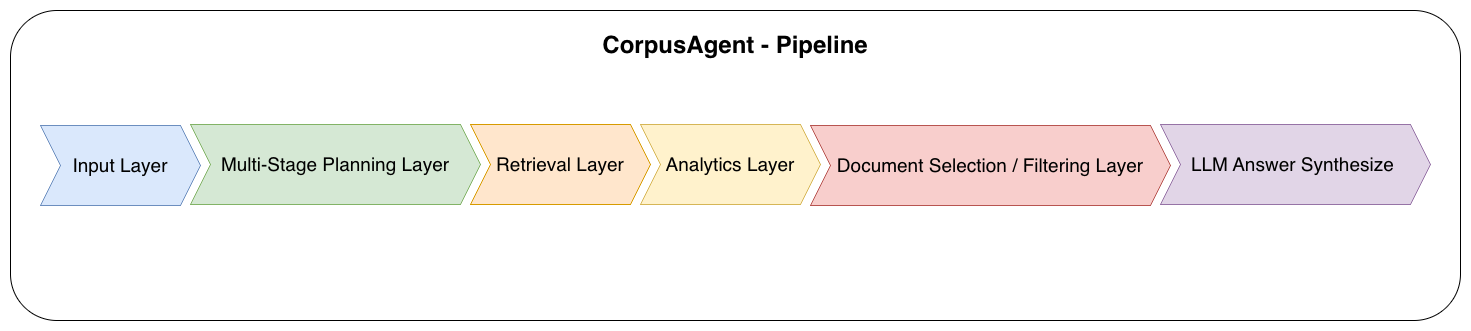
\includegraphics[width=1\textwidth]{Figures/Pipeline-Overview.png}
    \caption{Pipeline Overview (own illustration)}
    \label{fig:pipeline-overview}
\end{figure}

This thesis proposes a modular, multi-stage processing pipeline as illustrated in Figure \ref{fig:pipeline-overview}. The Pipeline of the CorpusAgent system is designed to answer complex, temporally-aware analytic questions over a large corpus of documents, specifically news articles. With such large datasets, it is infeasible to load all data into a large language model (LLM) prompt due to context length limitations. Therefore, the system breaks down the processing into several stages, each handled by specialized modules. Each of these layers is responsible for a specific transformation or decision step.

The core idea behind this architecture is to separate planning, retrieval, analysis, filtering and synthesis into independent stages. The separation of these stages allows for better scalability, maintainability, and the ability to swap out components as needed. Each layer incrementally refines the data, starting from a raw user query, progressing through structured retrieval and analytics processing and culminating in a final synthesized answer.

As this concept of ours is still experimental, we tried to structure the system as modularly as possible, so that individual components of the pipeline can be replaced or improved independently with different be it retrieval strategies, LLM models, or analytic techniques. The following section will describe each of these layers in detail, explaining their roles, inputs, outputs, and interactions with other components in the system.


%-----------------------------------
% Pipeline Layers
%-----------------------------------
\section{Pipeline Architecture}

The CorpusAgent pipeline is composed of a sequence of logically separated layers, each responsible for a specific aspect of the overall processing workflow. The layers are executed in a predefined order, where the output of one layer serves as the input for the next. This layered design allows complex analytical tasks to be decomposed into smaller, more manageable steps, improving transparency and enabling targeted evaluation of individual components.

In the following subsections, each pipeline layer is described in detail. For each layer, its purpose, inputs, outputs, and interactions with other layers are explained.

%-----------------------------------
% Input Layer
%-----------------------------------
\subsection{Input Layer}

\begin{figure}[ht]
    \centering
    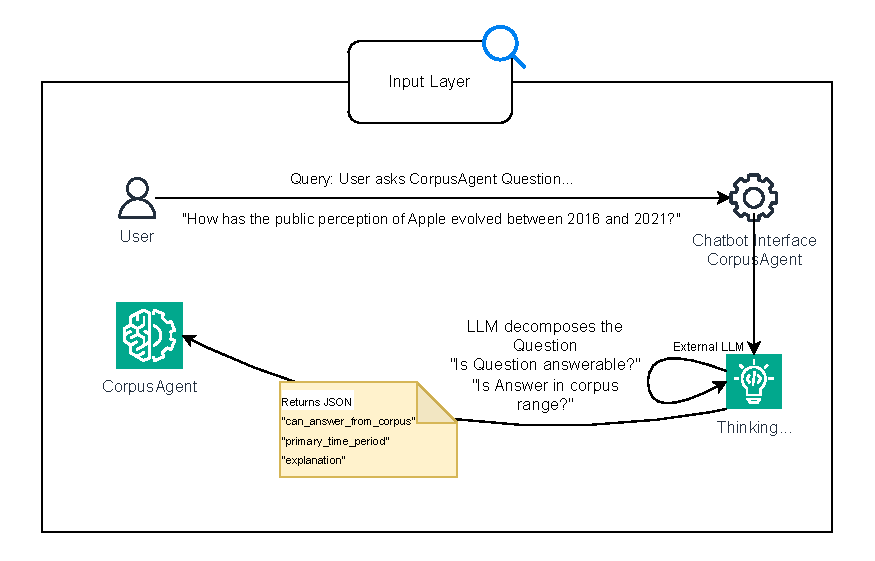
\includegraphics[width=1\textwidth]{Figures/input-layer.pdf}
    \caption{Input Layer (own illustration)}
    \label{fig:input-layer}
\end{figure}

The entry point of the CorpusAgent system is the Input Layer, as illustrated in Figure \ref{fig:input-layer}. It is responsible for receiving user queries, validating them, and performing any necessary preprocessing before passing them on to the subsequent layers.

The interaction begins when a user submits a natural language question through the chatbot interface of our CorpusAgent system. These questions are typically high-level analytical queries that may span over mutliple years and require aggregation or interpretation over a large corpus of documents.

Upon receiving a query, the Input Layer forwards it to an either external or internal Large Language Model (LLM) for an initial reasoning step. At this stage, the LLM does not attempt to generate a final answer. Instead, it performs a lightweight decomposition and feasibility assessment of the query. Specifically, it evaluates whether the question falls within the temporal and thematic scope of the indexed data.

The motivation behind this design decision is to introduce an explicit reasoning and validation step at the very beginning of the pipeline. By performing an initial feasibility assessment, the system can identify questions that cannot be meaningfully answered using the available corpus, for example due to missing temporal coverage or insufficient data. This early filtering prevents unnecessary downstream processing and ensures that subsequent pipeline stages operate only on well-scoped and answerable queries.

The outcome of the assessment is a structured JSON format containing whether the question is answerable, the primary time period of interest and a short explanation justifying the decision.



%-----------------------------------
% Multi-Stage Planning Layer
%-----------------------------------

\subsection{Multi-Stage Planning Layer}
\label{PipelinePlanningLayer}

\begin{figure}[ht]
    \centering
    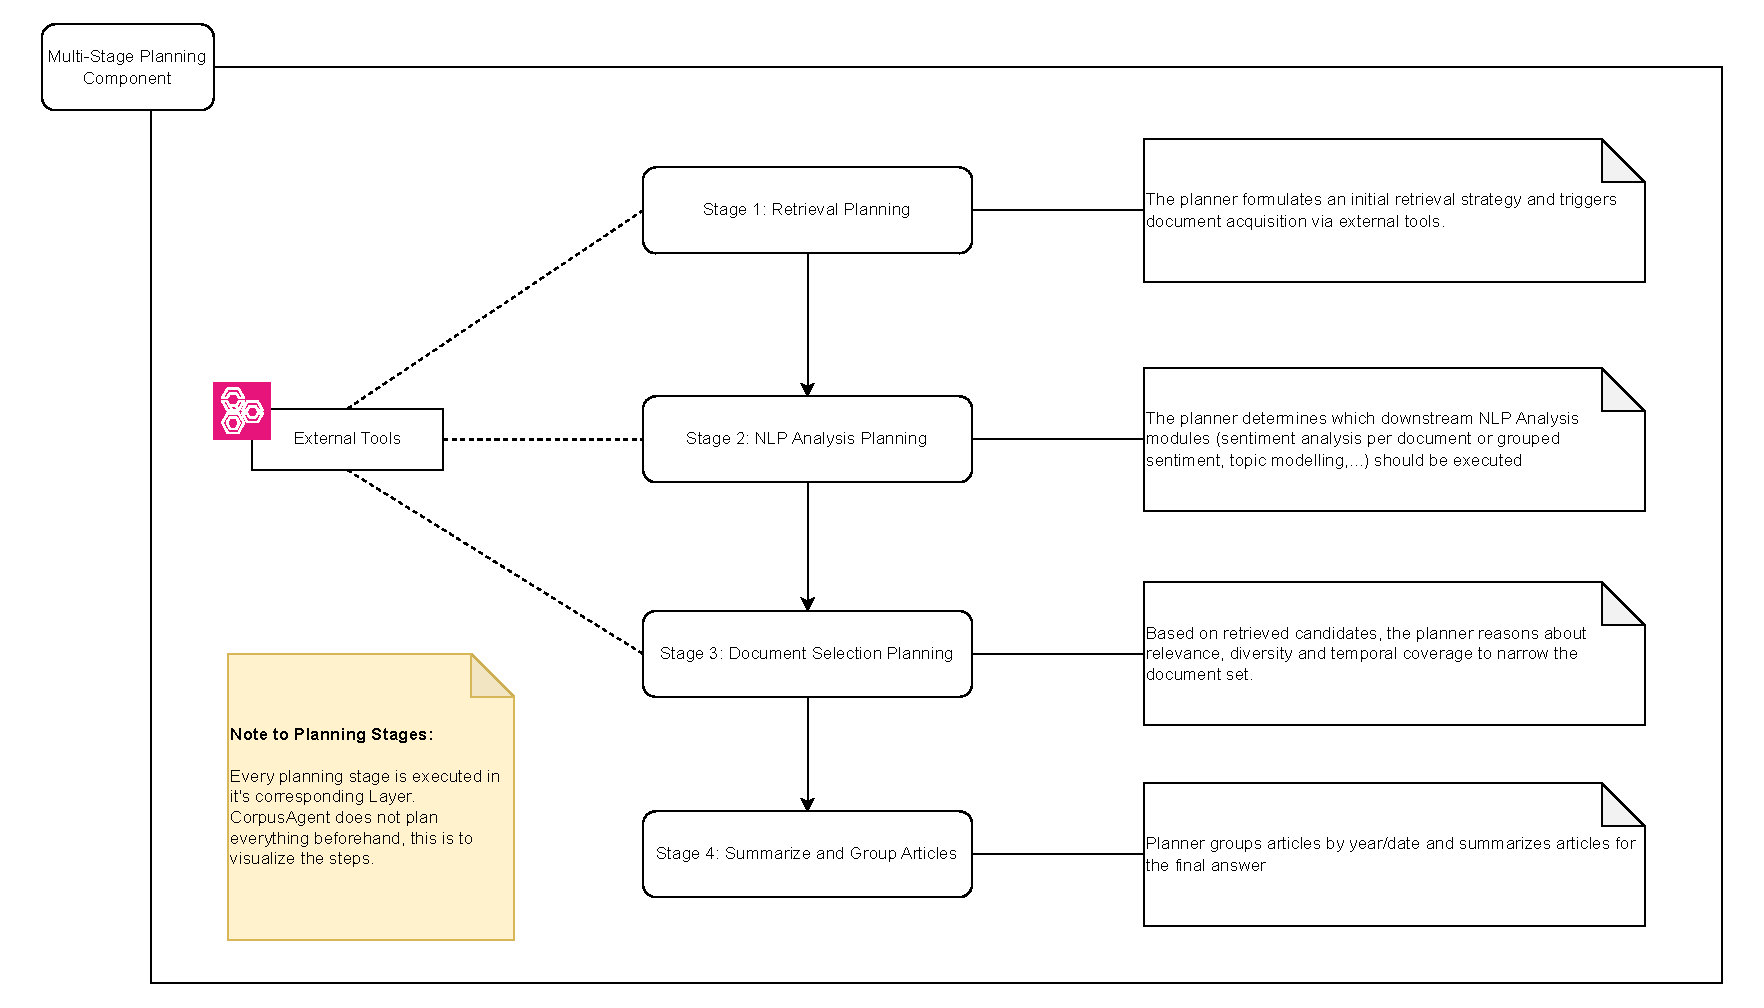
\includegraphics[width=1\textwidth]{Figures/planning-layer.pdf}
    \caption{Planning Layer (own illustration)}
    \label{fig:planning-layer}
\end{figure}

The Multi-Stage Planning Layer is responsible for orchestrating the overall problem-solving strategy of the CorpusAgent systeem. Contrary to the other layers, this layer is rather integrated into each of the other layers instead of being a standalone module as illustrated in Figure \ref{fig:planning-layer}. Rather than following a fixed, hard-coded execution path, this module introduces an agentic control mechanism in which a Large Language Model (LLM) dynamically determines how a given query should be processed across the various pipeline layers.

At this stage, the LLM is provided with a set of available external tools it can execute. These tools consist of function calls such as retrieval, natural language processing (NLP) analyses, document filtering and answer synthesis. However, the specific decisions regarding which tools to invoke, in what order and how many times are delegated to the LLM itself. Rather than a rigid sequence of operations, the planning layer enables a flexible, adaptive approach where the LLM can iteratively refine its strategy based on intermediate results. This design choice allows the system to adapt its strategy to the nature and complexity of the input query and can lead to multiple strategies for the same question.

What makes this approach particularly powerful is that the decision-making authority is not limited to a single planning step. Instead, the LLM is invoked after each major pipeline stage to reassess the current state of the task and determine the next best approach.

Each stage operates as a controlled execution step, while the overall reasing flow is handled by the LLM's conextual understanding ot the task. This agentic, multi-stage planning approach enables our system to handle a wide range of analytic queries with varying results.

The first concrete execution step is determined by the LLM is the retrieval of the relevant documents, which is described in the next section.


\subsection{Retrieval Layer}

\begin{figure}[ht]
    \centering
    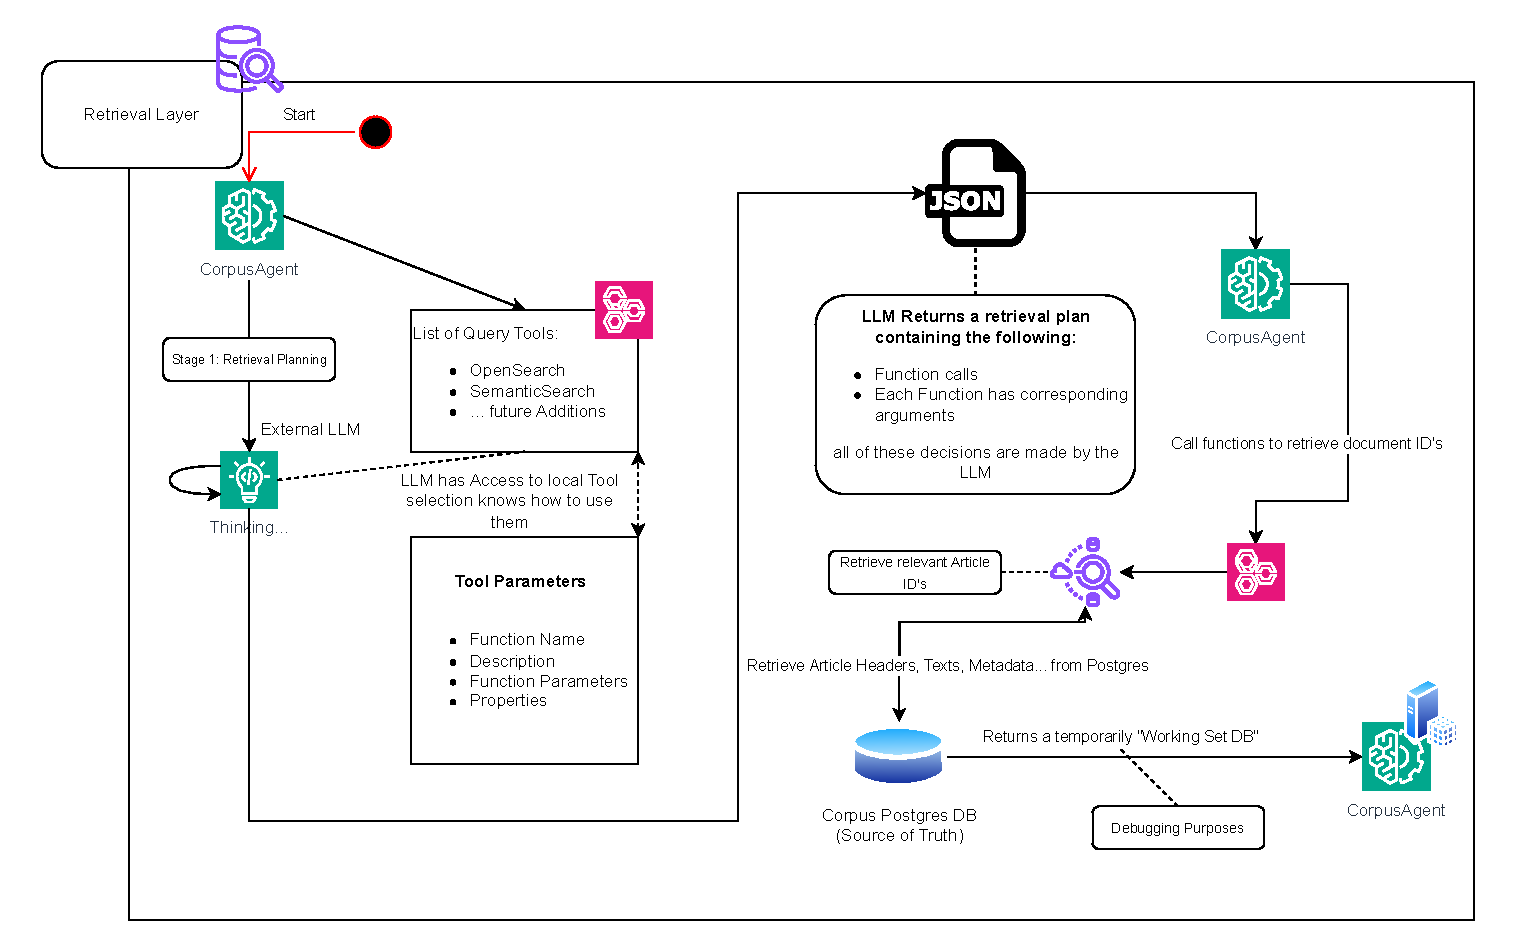
\includegraphics[width=1\textwidth]{Figures/retrieval-layer.pdf}
    \caption{Retrieval Layer (own illustration)}
    \label{fig:retrieval-layer}
\end{figure}

The Retrieval Layer is responsible for identifying and collecting a set of documents that are potentially relevant to the user’s query. Its primary goal is to efficiently reduce the overall corpus to a manageable subset that can be further analyzed by subsequent pipeline stages. An overview of this process is illustrated in Figure \ref{fig:retrieval-layer}.

As like with the other layers, the retrieval process is guided by the retrieval planning decisions made by the Large Language Model. The LLM determines here the appropriate retrieval strategy based on the user query and provided toolset. Rather than directly accessing the data itself, the LLM generates a structured retrieval plan in the form of one or more function calls. These function calls specify which retrieval tools should be used, the corresponding query expressions, and additional parameters such as the number of documents to return. All retrieval related decisions, including whether multiple retrieval calls are required, for example to cover different time periods, are made by the LLM.

Currently, the primary retrieval backend is OpenSearch, which is used to index the news corpus and enable fast full-text search. OpenSearch is based on the Lucene engine and relies on inverted indices, allowing keyword-based queries to be executed significantly faster than traditional relational database text matching. In preliminary experiments, this approach was empirically validated by comparing OpenSearch queries against SQL-based text search using \texttt{LIKE} expressions in PostgreSQL, where OpenSearch consistently produced substantially faster query execution times for large text collections. Which is to be expected given the underlying indexing mechanisms.

The use of OpenSearch at this stage is not only motivated by performance considerations but also by extensibility. The retrieval interface is designed in such a manner, such that additional retrieval mechanisms such as semantic vector search or alternative indexing systems can be integrated in the future without requiring fundamental changes to the architecture.

An example of a retrieval function call generated by the LLM is shown below:

\begin{lstlisting}[language=json, caption={Example OpenSearch retrieval function call}, label={lst:opensearch-call}]
{
  "id": "call_VBCxxwHwvAluJHuoMOrdC6iF",
  "type": "function",
  "function": {
    "name": "search_opensearch",
    "arguments": {
      "query": "Bitcoin (\"public perception\" OR \"public opinion\" OR sentiment OR adoption OR \"mainstream\" OR bubble OR scam OR regulation OR investment) 2016",
      "top_k": 50
    }
  }
}
\end{lstlisting}

Such function calls like the one shown in Listing \ref{lst:opensearch-call} are generated by the LLM based on the entire context provided to it, including the user query. These are then returned to the CorpusAgent in a structured JSON format. The CorpusAgent executes all the specified function calls and collects the resulting documents.

The system eomploys both a PostgreSQL database and an OpenSearch index to balance data integrity, flexibility and retrieval performance. Here we use PostgreSQL as the primary data store and authoritative source of truth for all news articles and associated metadata. The reason behind this design choice is to ensure that the complete and consistent dataset is maintained in a robust relational database system.

Using a relational database as the main data source also provides more flexibility for future extensions of the news corpus or completely new datasets. Different datasets may have additional metadata beyond the basic fields such as headlines and article text. Such attributes may be relevant for downstream analysis or filtering steps but not necessarily suitable or required for indexing in OpenSearch. Maintaining these attributes in PostgreSQL allows the system to evolve without requiring changes to the indexing structure.

Therefore OpenSearch is used as a secondary, specialized component optimized for large scale text retrieval. Separating these concerns allows the system to combine the strengths of both technologies, having a reliable primary data store while leveraging the performance benefits of a dedicated search engine for text retrieval tasks.

In addition to these persisent data stores, the system maintains a temporary, per-run working database that archives all retrieved documents and intermediate NLP outputs generated during a single pipeline execution. The purpose of this temporary dataset is primarily intended for debugging, analysis and result validation. Given the exploratory and analytical nature of the task, determining whether a generated answer is correct is inherently challenging. Instead of relying solely on the final answers, this design allows the the user to inspect the entire processing history, including which documents were retrieved and how they were analyzed. This transparency facilitates error analysis and helps identify potential issues in the retrieval or processing steps. Not to mention, it allows the user to assess whether the final answer is grounded in the retrieved evidence rahter than relying on unsupported or hallucinated information.

% TODO : Add a SQL Database Schema Figure
\subsection{Analytics Layer}

\begin{figure}[ht]
    \centering
    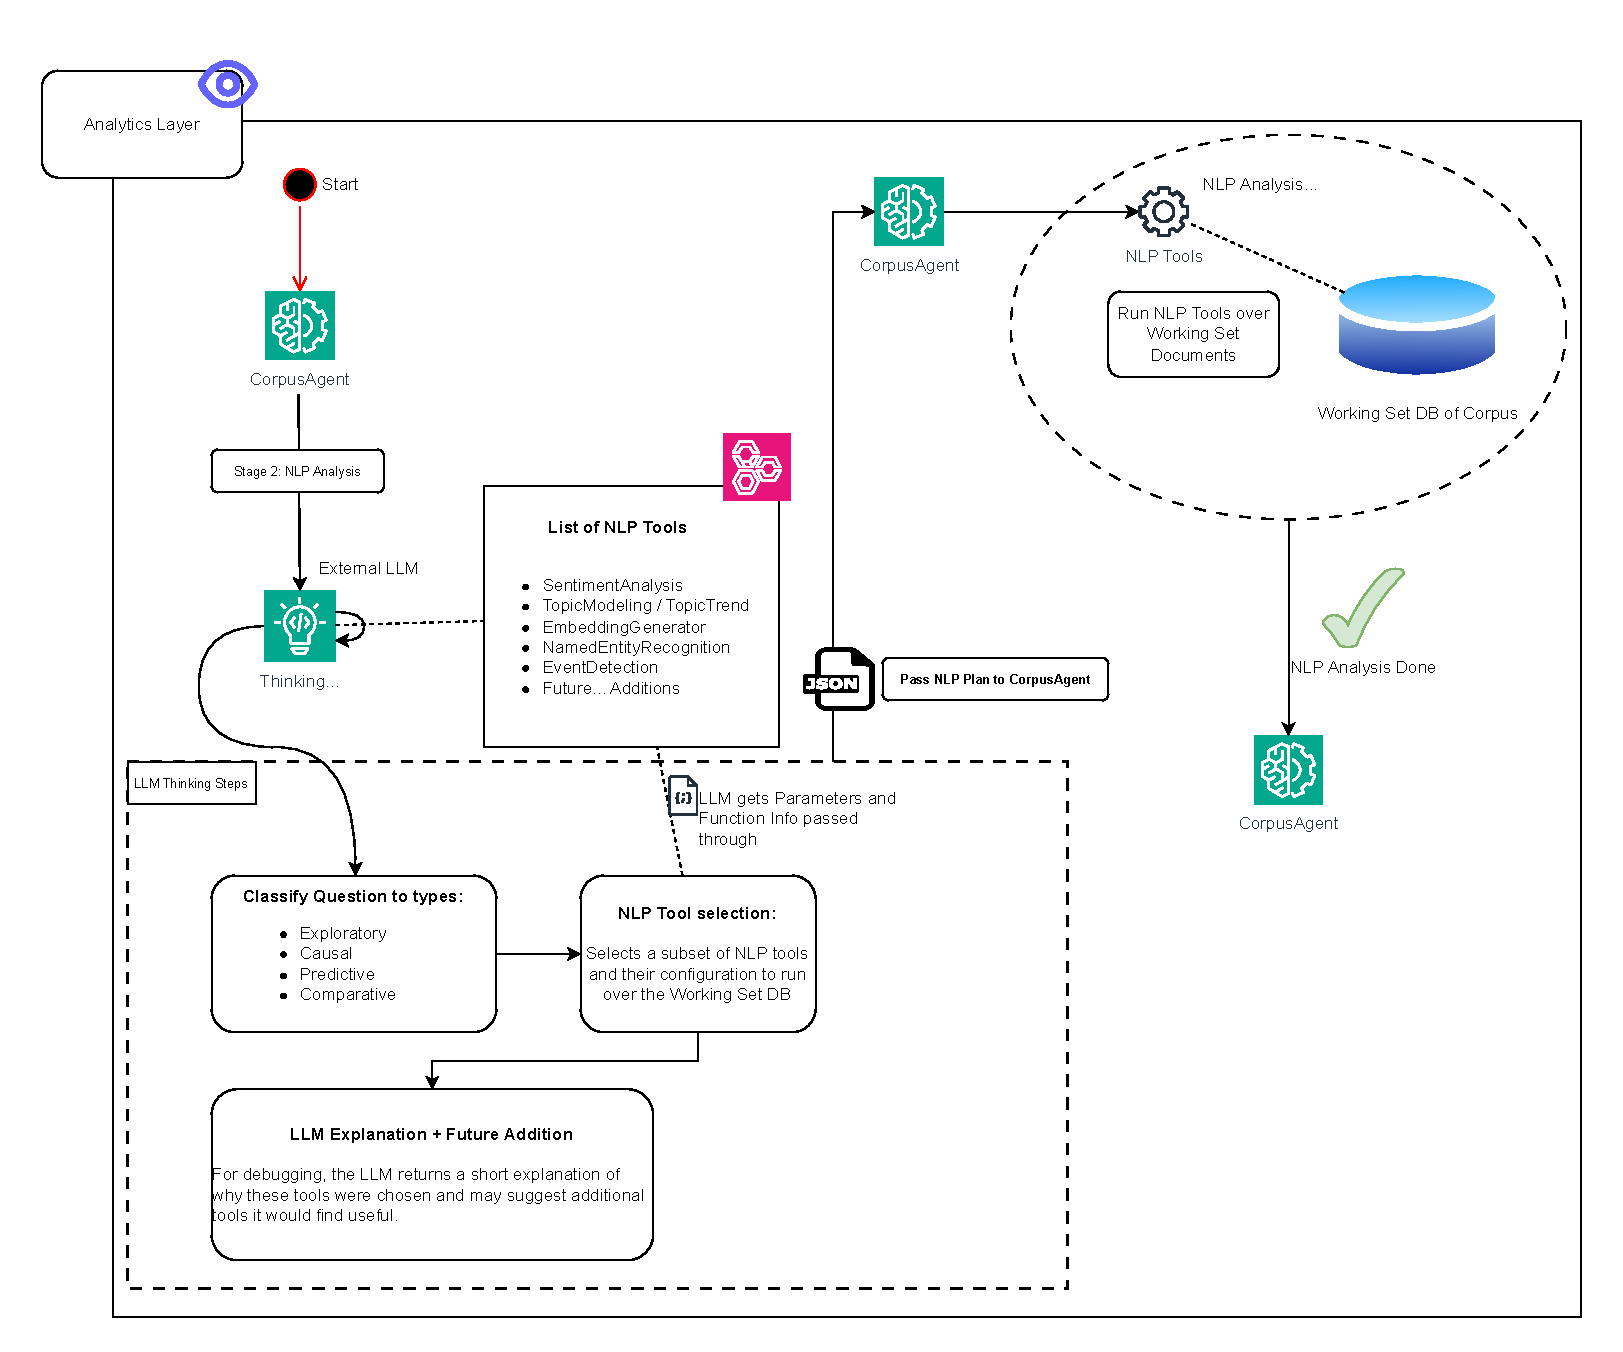
\includegraphics[width=1\textwidth]{Figures/analytics-layer.pdf}
    \caption{Analytics Layer (own illustration)}
    \label{fig:analytics-layer}
\end{figure}

The Analytics Layer is responsible for applying targeted natural language processing (NLP) methods to the working set of documents retrieved in the previous stage. Primarily, its objective is to extract structured signals from unstructured text that support higher-level analytical reasoning, such as identifying trends, sentiments, entities, or events over time. An overview of this process is illustrated in Figure~\ref{fig:analytics-layer}.

At the beginning of this layer, the Large Language Model (LLM), guided by the Multi-Stage Planning Layer, determines which analytical tools are appropriate for the given query. Rather than executing all available NLP methods indiscriminately, the system adopts a selective approach in which the LLM first classifies the nature of the question, for example as exploratory, comparative, predictive, or causal. Based on this classification, the LLM selects a subset of NLP tools and configures their parameters accordingly. Additionally, we prompt the LLM to provide a brief explanation of why specific tools were chosen, which serves as documentation for the analytical strategy. Furthermore we ask the LLM to suggest any additional tools that could be relevant for future iterations, even if they are not executed in the current run.


The applied NLP methods represent well-established techniques for extracting structured information from large text corpora, including sentiment analysis, topic modeling, named entity recognition, and event detection. Such techniques have been extensively studied and applied in prior work on text analytics and information extraction \cite{jurafsky2023slp, blei2003lda, pang2008sentiment}.

Currently in this concept phase, we have only mocked the actual implementation of these NLP tools. However, in a fully realized system, each selected tool would be executed over the temporary working dataset produced by the Retrieval Layer. The outputs of these analyses would then be stored back into the working database, enriching the document set with structured annotations that can be leveraged in subsequent processing steps.

Depending on the type of analysis, the NLP Outputs are either stored per article (e.g., sentiment scores, named entities) or when there are cross-document results (e.g., topics, event clusters), they are stored in separate tables linked to the relevant articles. This structured storage approach allows for efficient querying and aggregation of analytical results during later stages of the pipeline.


All selected NLP tools are executed over the temporary working dataset produced by the Retrieval Layer. By operating on this reduced document set, the system avoids unnecessary computation over the full corpus while still retaining sufficient contextual coverage for meaningful analysis. The LLM specifies tool selections, execution order, and configuration parameters in a structured JSON format, which is subsequently interpreted and executed by the CorpusAgent.

Once all selected NLP analyses have been completed, the enriched working dataset is passed to the Document Selection and Filtering Layer for further refinement.

\pagebreak

\subsection{Document Selection / Filtering Layer}

\begin{figure}[ht]
    \centering
    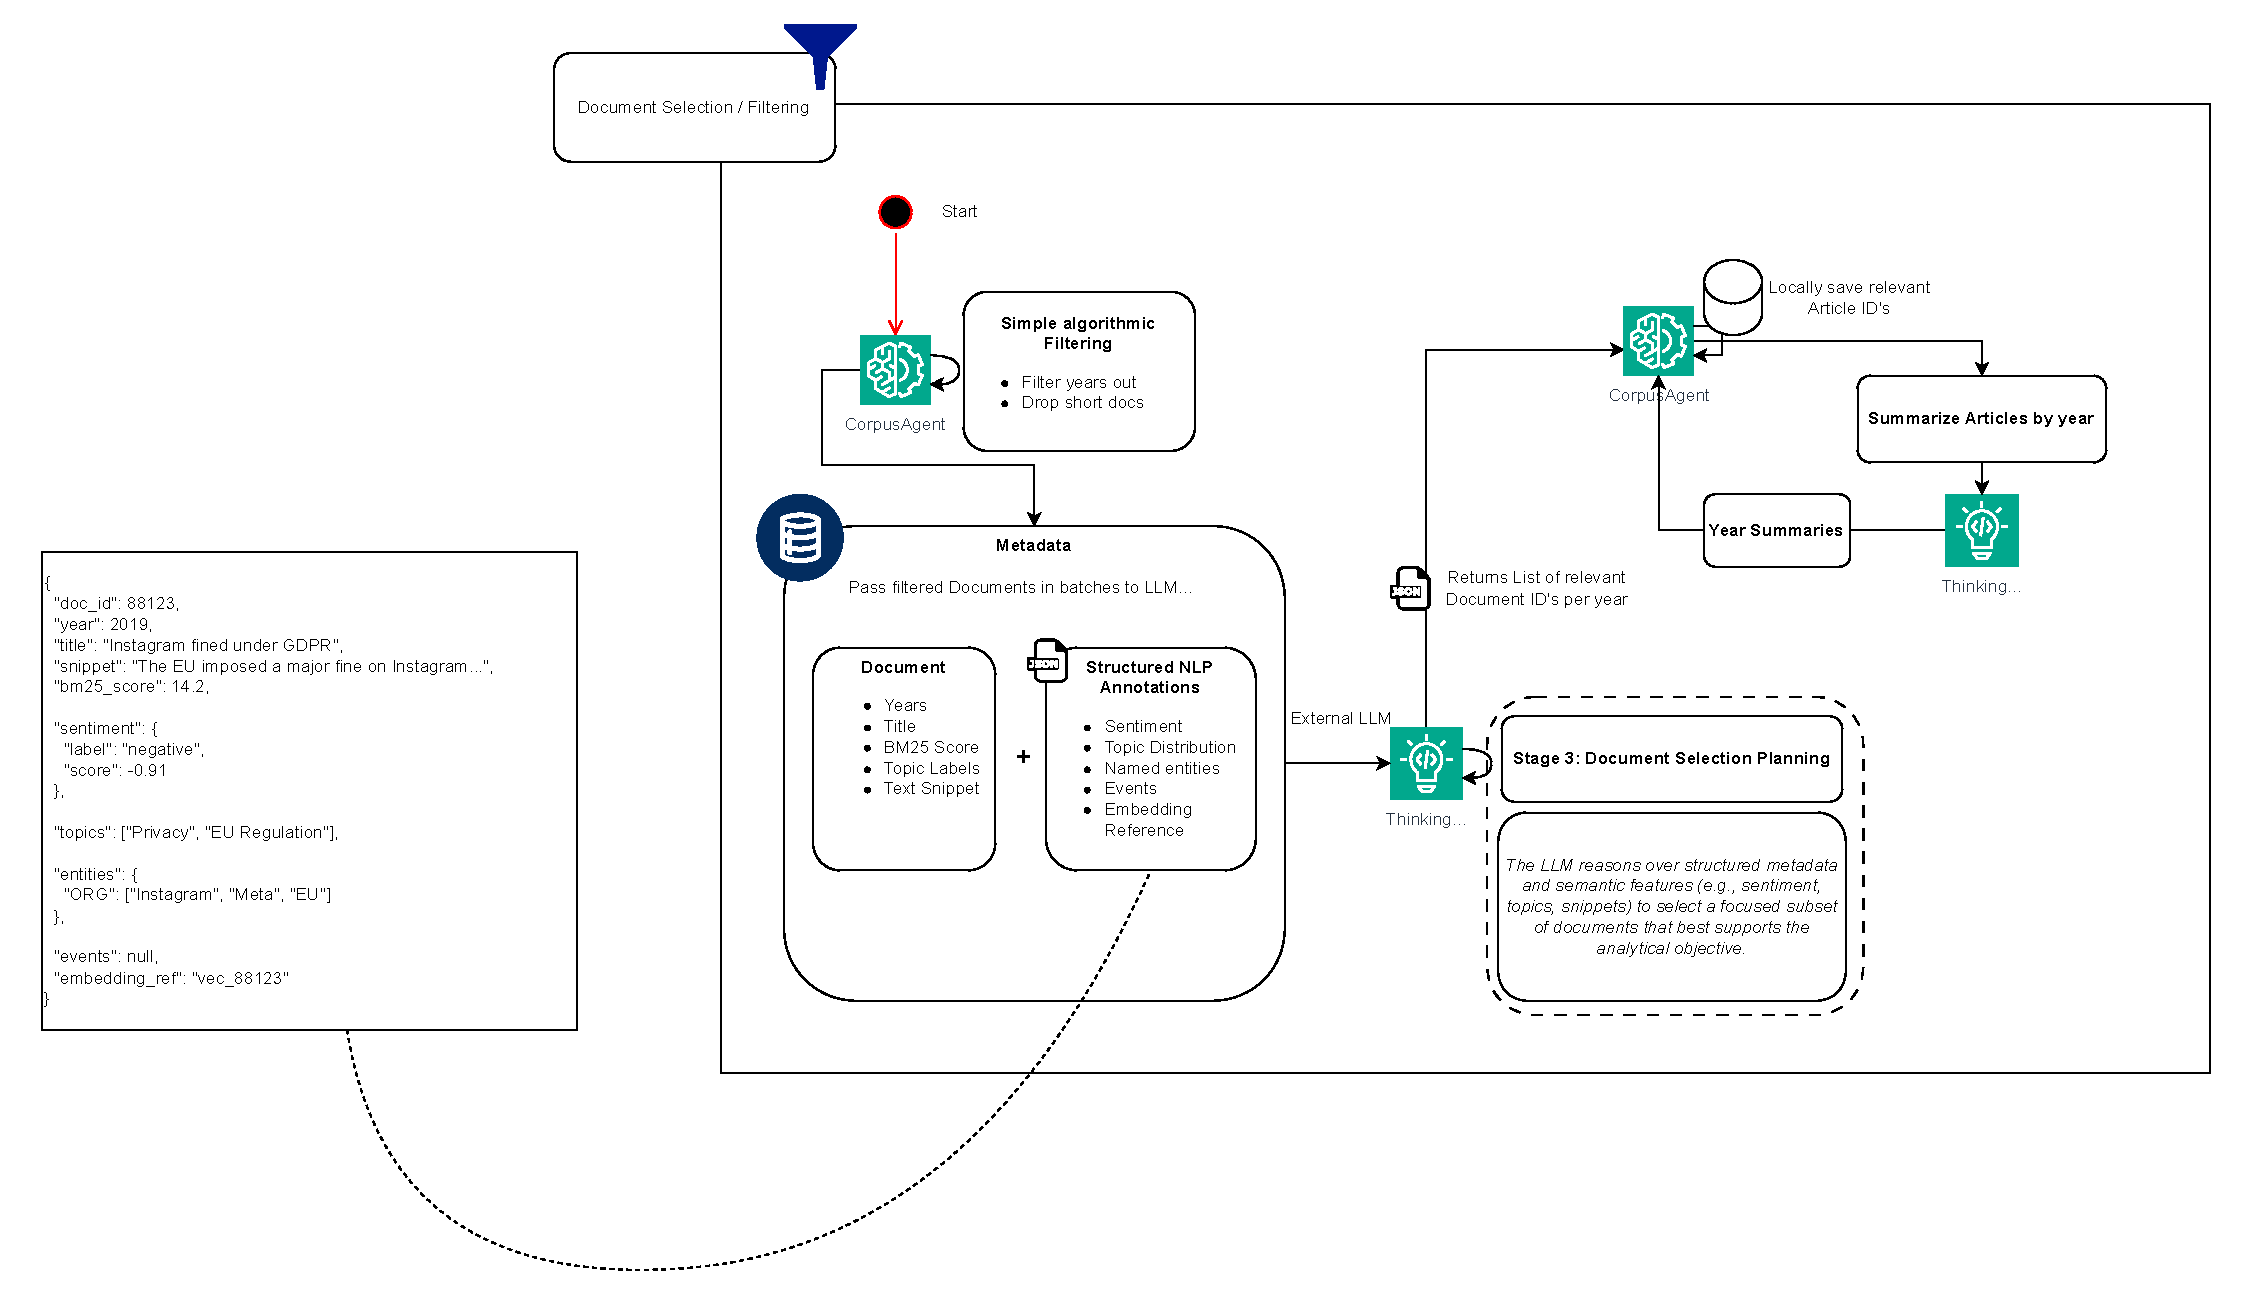
\includegraphics[width=1\textwidth]{Figures/document-filtering.pdf}
    \caption{Document Selection / Filtering Layer (own illustration)}
    \label{fig:document-filtering-layer}
\end{figure}

The Document Selection and Filtering Layer is responsible for refining the analytically enriched working dataset to a focused subset of documents that most effectively support the final answer synthesis. Previous pipeline stages were primarily concerned with broad retrieval and comprehensive analysis. In contrast, this layer aims to distill the dataset down to the most relevant and informative documents. An overview of this process is illustrated in Figure \ref{fig:document-filtering-layer}.

Here the filtering process first off begins with a lightweight, deterministic pre-filtering step directly inside the CorpusAgent. This step applies simple algorithmic criteria to eliminate documents that are clearly irrelevant or low-quality. Such criteria may include removing duplicates, filtering out articles below a certain length, or excluding documents that do not meet the time horizon of the task. This initial pruning helps reduce noise and focuses subsequent processing on a more manageable set of candidates.

After this initial pre-filtering, the refined working dataset is represented in a structured format that combines retrieved metadata and analytical annotations from the analytical layer. This structured representation includes among other attributes, the publication year, title, full article text, retrieval score (e.g. BM25), sentiment score and label and identified named entities. These attributes can vary depending on the specific NLP tools applied in the previous layer.

In this next step, the CorpusAgent forwards these document representations in batches to the Large Language Model (LLM). Instead of selecting documents based on fixed attributes like retrieval scores or sentiment thresholds, we prompt the LLM to reason with the initial user query in mind, to determine which documents are most important to answering the question.

As a result, the LLM evalutes in each batch which documents are most relevant and informative for the specific analytical task. The selected document IDs are then returned to the CorpusAgent in a structured JSON format with once again an explanation of why these documents were chosen. Inside the temporary working database, the CorpusAgent marks these documents as selected for inclusion in the final answer synthesis.

Finally, once all documents have been processed, the CorpusAgent once again prompts the LLM to generate a summary of each year represented in the selected documents. These yearly summaries provide a concise overview of the key themes, events, and trends identified in the filtered dataset. They also serve to reduce the overall context length required for the final answer synthesis step, as only the summaries rather than the full articles need to be considered.

Our motivation behind this layer was to introduce a human-like judgment step into the pipeline. Rather than relying solely on algorithmic criteria, we leverage the LLM's contextual understanding to make nuanced decisions about document relevance. This approach allows the system to adaptively focus on the most pertinent information for each unique query, ultimately improving the quality and accuracy of the final synthesized answers.

With the selected documents and yearly summaries prepared, the pipeline is now ready to proceed to the final stage: LLM Answer Synthesis.

\subsection{LLM Answer Synthesis}

\begin{figure}[ht]
    \centering
    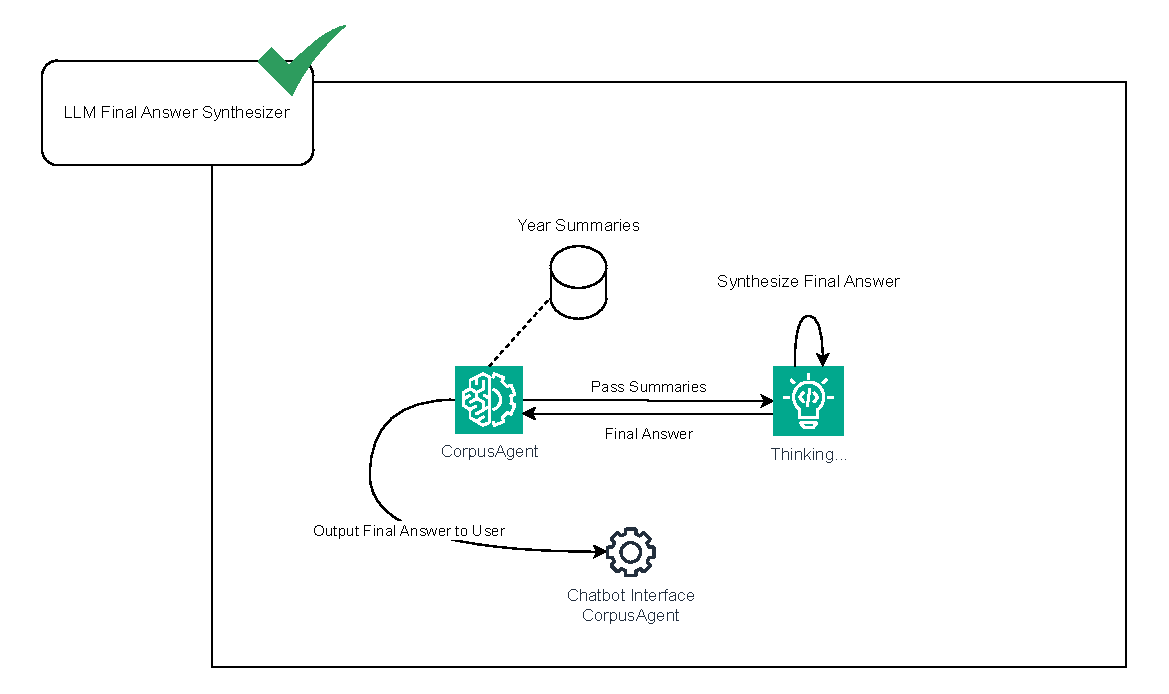
\includegraphics[width=1\textwidth]{Figures/final-synthesize.pdf}
    \caption{LLM Answer Synthesis Layer (own illustration)}
    \label{fig:llm-answer-synthesis-layer}
\end{figure}

The final stage of the CorpusAgent pipeline is the LLM Answer Synthesis Layer, as illustrated in Figure \ref{fig:llm-answer-synthesis-layer}. This layer is responsible for generating a coherent, well-structured answer to the user's original query based on the refined set of documents and analytical insights produced by the preceding layers. Combined with the input layer, these two layers are the only parts of the pipeline that directly interact with the user. At this point, the system relies solely on the condensed, temporally organized summaries that capture the most relevant information extracted from the corpus.

The CorpusAgent passes the yearly summaries derived from the Documen Selection phase before to the LLM along with the original user query. Additionally, we provide even further context if available, such as NLP outputs that may span over multiple documents (e.g., identified trends or events). The LLM is then prompted to synthesize this information into a comprehensive answer that directly addresses the user's question.

The synthesis process focuses on identifying overarching patterns, temporal developments, and meaningful comparisons across time periods. For example, shifts in sentiment, changes in dominant topics, or the emergence of new narratives can be explicitly highlighted and related back to the original analytical question. The resulting output is a single, consolidated answer that integrates insights across all relevant years.

Finally, the synthesized answer is returned to the user through the chatbot interface of the CorpusAgent system. By separating answer generation from retrieval, analysis, and document selection, this layer provides a clear abstraction boundary and ensures that the final response can be traced back to specific intermediate representations. This transparency is crucial for validating the correctness and reliability of the generated answers, especially in complex analytical scenarios.

\pagebreak

%-----------------------------------
% Visualization Playground
%-----------------------------------

\section{Visualization Playground (Auxiliary Component)}

\begin{figure}[ht]
    \centering
    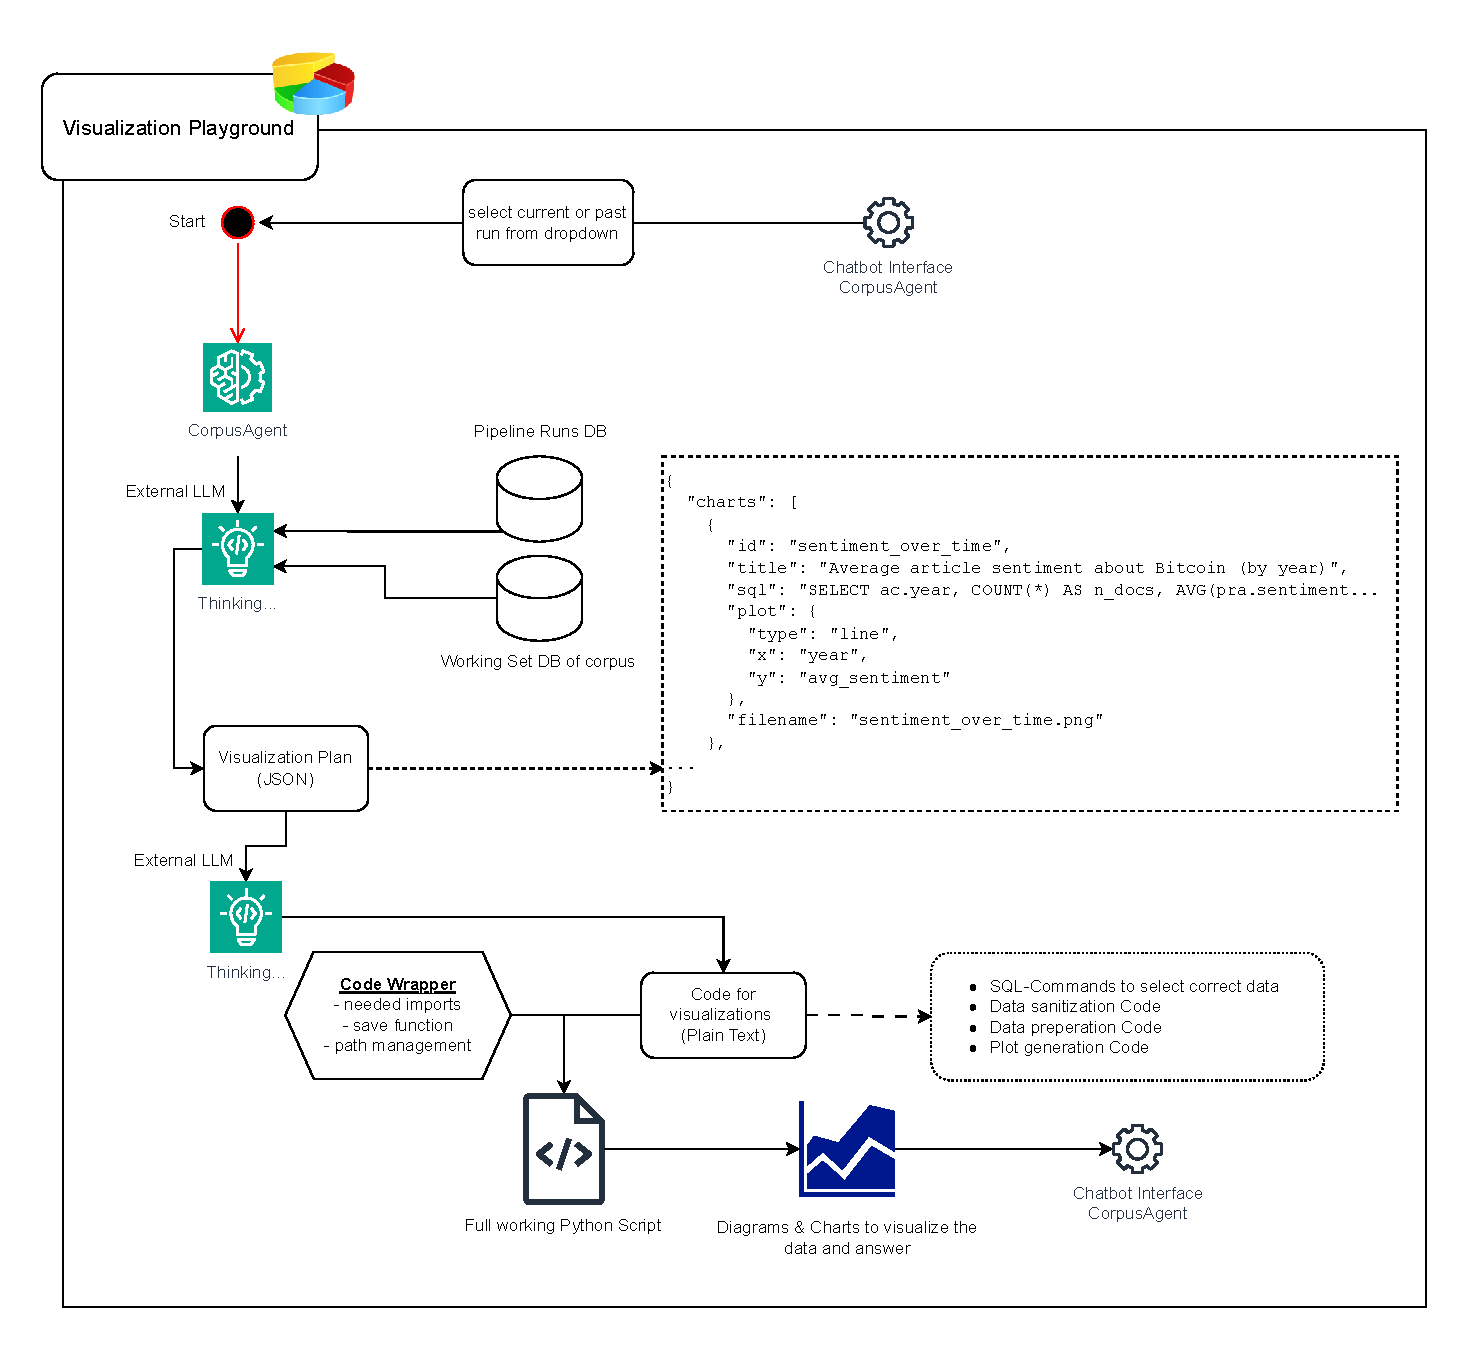
\includegraphics[width=1\textwidth]{Figures/visualization-playground.pdf}
    \caption{Visualization Playground (own illustration)}
    \label{fig:visualization-playground}
\end{figure}

The CorpusAgent pipeline is designed to answer complex analytical questions over large news corpora by decomposing the task into retrieval, analysis, filtering, and synthesis stages. \\
However, corpus-level analytics are difficult to validate purely from a final textual answer. Users typically need to inspect temporal trends, distributions, and supporting evidence to judge whether the answer is grounded in the retrieved material. Also, visualizations can help communicate complex patterns more effectively than text alone.
To support this requirement, we implemented a Visualization Playground as an auxiliary component that generates plots and diagrams on demand for a selected pipeline run.
Conceptually, the playground consumes two persistent information sources:

\begin{itemize}
    \item The authoritative corpus and per-run working set stored in PostgreSQL
    \item The pipeline run metadata and outputs (e.g., question, final answer, and structured intermediate artifacts) stored in a separate run database
\end{itemize}

Based on this input, the system produces a visualization plan (structured JSON), generates executable plotting code, and renders the resulting images as reproducible artifacts that can be inspected inside the interface.

This design mirrors the high-level workflow shown in the Figure \ref{fig:visualization-playground}: an LLM produces a JSON visualization specification and plotting code which is executed to create charts saved as run artifacts.

\subsection{Data Sources and Run Selection}

The playground is run-centric: the user selects a run\_id corresponding to a previously executed pipeline run. \\
The implementation provides a small run management module that lists recent runs and fetches detailed run information from the pipeline\_runs table, including fields such as question, final\_answer, and additional stored debug artifacts. These run-level fields serve two purposes:

\begin{enumerate}
    \item Semantic context for the visualization planner and code generator (the LLM is conditioned on what the run was trying to answer).
    \item Traceability since produced charts can always be linked back to an immutable run identifier.
\end{enumerate}

In addition to run metadata, the playground queries the per-run working dataset stored in pipeline\_run\_articles (linked to the main corpus table article\_corpus). The design intentionally queries only a reduced, run-specific slice rather than the entire corpus to keep visualization computation bounded and directly relevant to the specific question.

\begin{lstlisting}[caption={Example DB schema summary}, label={lst:db-schema}]
article_corpus(id bigint, year smallint, source_domain text, title text, body text)

pipeline_run_articles(run_id uuid, question text, article_id bigint, rank integer, os_score real, sentiment_score real, relevance_score real, extra_metadata jsonb)

pipeline_runs(run_id uuid, question text, nlp_plan jsonb, mocked_tool_outputs jsonb, final_answer text, created_at timestamp with time zone)
\end{lstlisting}

\subsection{LLM-Based Visualization Planning}

The first step is planning: given (question, final\_answer, run\_id), the planner asks the LLM to propose a set of charts expressed as a JSON structure. \\
Each chart entry contains: a stable identifier \textit{id}, a human-readable \textit{title}, an SQL query string \textit{sql}, a minimal plot specification \textit{plot} (e.g. type, x, y) and an output \textit{filename} (PNG).

This plan is explicitly constrained to valid JSON via structured response formatting (JSON object), which makes downstream handling deterministic (e.g., rendering the plan in the UI, validating presence of required fields). The planner prompt also injects a compact schema summary so the model does not need to guess table/column names.

The full JSON plan can be inspected before proceeding to code generation, allowing the user to verify that the proposed charts align with their expectations.

\begin{lstlisting}[caption={Example Visualization Plan JSON}, label={lst:viz-plan}]
{
    "charts": [
        index : {
            "id": "...",
            "title": "...",
            "sql": "... WHERE pra.run_id = :run_id ...",
            "plot": { "type": "line|bar", "x": "...", "y": "..." },
            "filename": "...png"
        },
        ...
    ]
}
\end{lstlisting}

A key design concern is the presence of \textit{extra\_metadata} stored as JSONB, which varies between runs. To reduce hallucinated JSON keys, the planner additionally includes a glimpse of observed JSON key paths and examples extracted from the selected run. The LLM is instructed to use only those keys and to query JSONB via Postgres JSON operators when needed.

\subsection{LLM-Based Code Generation}

The visualization plan is intentionally lightweight. It is primarily meant for transparency and for guiding the next step: code generation. \\
In the second step, the system prompts the LLM to generate Python plotting code that queries the PostgreSQL database and produces PNG charts using Matplotlib. The code generator is constrained through explicit rules, including:

\begin{itemize}
    \item return only Python code (no markdown)
    \item use Matplotlib (avoid additional plotting dependencies)
    \item obtain data via a provided \textit{query\_df(sql, params)} helper
    \item save output figures only through a provided \textit{save\_fig(fig, filename)} function
\end{itemize}

This separation (plan → code) is deliberate: the plan acts as a structured, inspectable intermediate representation, while the code step is responsible for the full procedural details (data preparation, grouping/aggregation, plotting, labeling, and exporting).
It also helps preventing hallucinated Code regarding paths, run\_id usage, and saving conventions.

\subsection{Controlled Execution and Artifact Management}

To execute LLM-generated code while keeping the system reproducible and debuggable, the playground runs the generated script via a wrapper-based execution mechanism:
\begin{enumerate}
    \item The user-generated code is written to an artifact directory under the selected run\_id.
    \item A wrapper script is created which injects:
          \begin{itemize}
              \item environment-backed values (RUN\_ID, OUT\_DIR)
              \item the database query helper query\_df
              \item and a constrained \textit{save\_fig} routine that validates .png filenames and writes output into OUT\_DIR
          \end{itemize}
    \item The wrapper is executed in a subprocess with an explicit timeout to prevent runaway code.
    \item Standard output/error are captured into log files.
    \item All produced PNGs are collected from the artifact directory and displayed in the interface.
\end{enumerate}

Artifacts are stored in a structured directory layout (e.g., artifacts/visuals/<run\_id>/...) to ensure that every generated visualization is reproducible and attributable to a run. \\
Since this feature is heavily volatile, due to LLM code generation, persisting the generated code and execution logs is also crucial for failure analysis: when plots fail to render (e.g., SQL errors, schema mismatches, missing fields), the developer can directly inspect the exact script, stdout, and stderr of the run.

\begin{lstlisting}[language=Python, caption={Safety and reproducibility wrapper for executing LLM-generated plotting code}, label={lst:code-exec-wrapper}]
import os
from pathlib import Path
import matplotlib.pyplot as plt

from viz.db import query_df  # SQLAlchemy-based query_df

# path setup
RUN_ID = os.environ.get("RUN_ID")
OUT_DIR = Path(os.environ.get("OUT_DIR", ".")).resolve()
OUT_DIR.mkdir(parents=True, exist_ok=True)

# constrained save_fig implementation
def save_fig(fig, filename: str) -> str:
    if not filename.endswith(".png"):
        raise ValueError("filename must end with .png")
    path = (OUT_DIR / filename).resolve()
    fig.savefig(path, dpi=160, bbox_inches="tight")
    plt.close(fig)
    return str(path)

# --- user code below ---
run_id = RUN_ID
{user_code}
\end{lstlisting}


% !TEX root = ../main.tex
%----------------------------------------------------------------------------------------

\chapter{Example Walkthrough} 
\label{ChapterExampleWalkthrough}

%----------------------------------------------------------------------------------------

The previous chapter described the CorpusAgent system from an architectural and methodological perspective, detailing the individual pipeline layers and their interactions. While this abstraction is necessary to understand the design rationale and technical capabilities of the system, it does not directly indicate how these components manifest in an actual system execution.

This chapter therefore provides an example walkthrough of the CorpusAgent interface from a system-level UI perspective. The walkthrough illustrates how the previously introduced architectural components are reflected in the interface and how they interact during a concrete pipeline run. \\
For each stage, the corresponding UI elements are presented alongside brief references to the underlying technical processes described in Chapter~\ref{ChapterMethodology}

\section{Step 1 - Entering a Question}

\begin{figure}[ht]
    \centering
    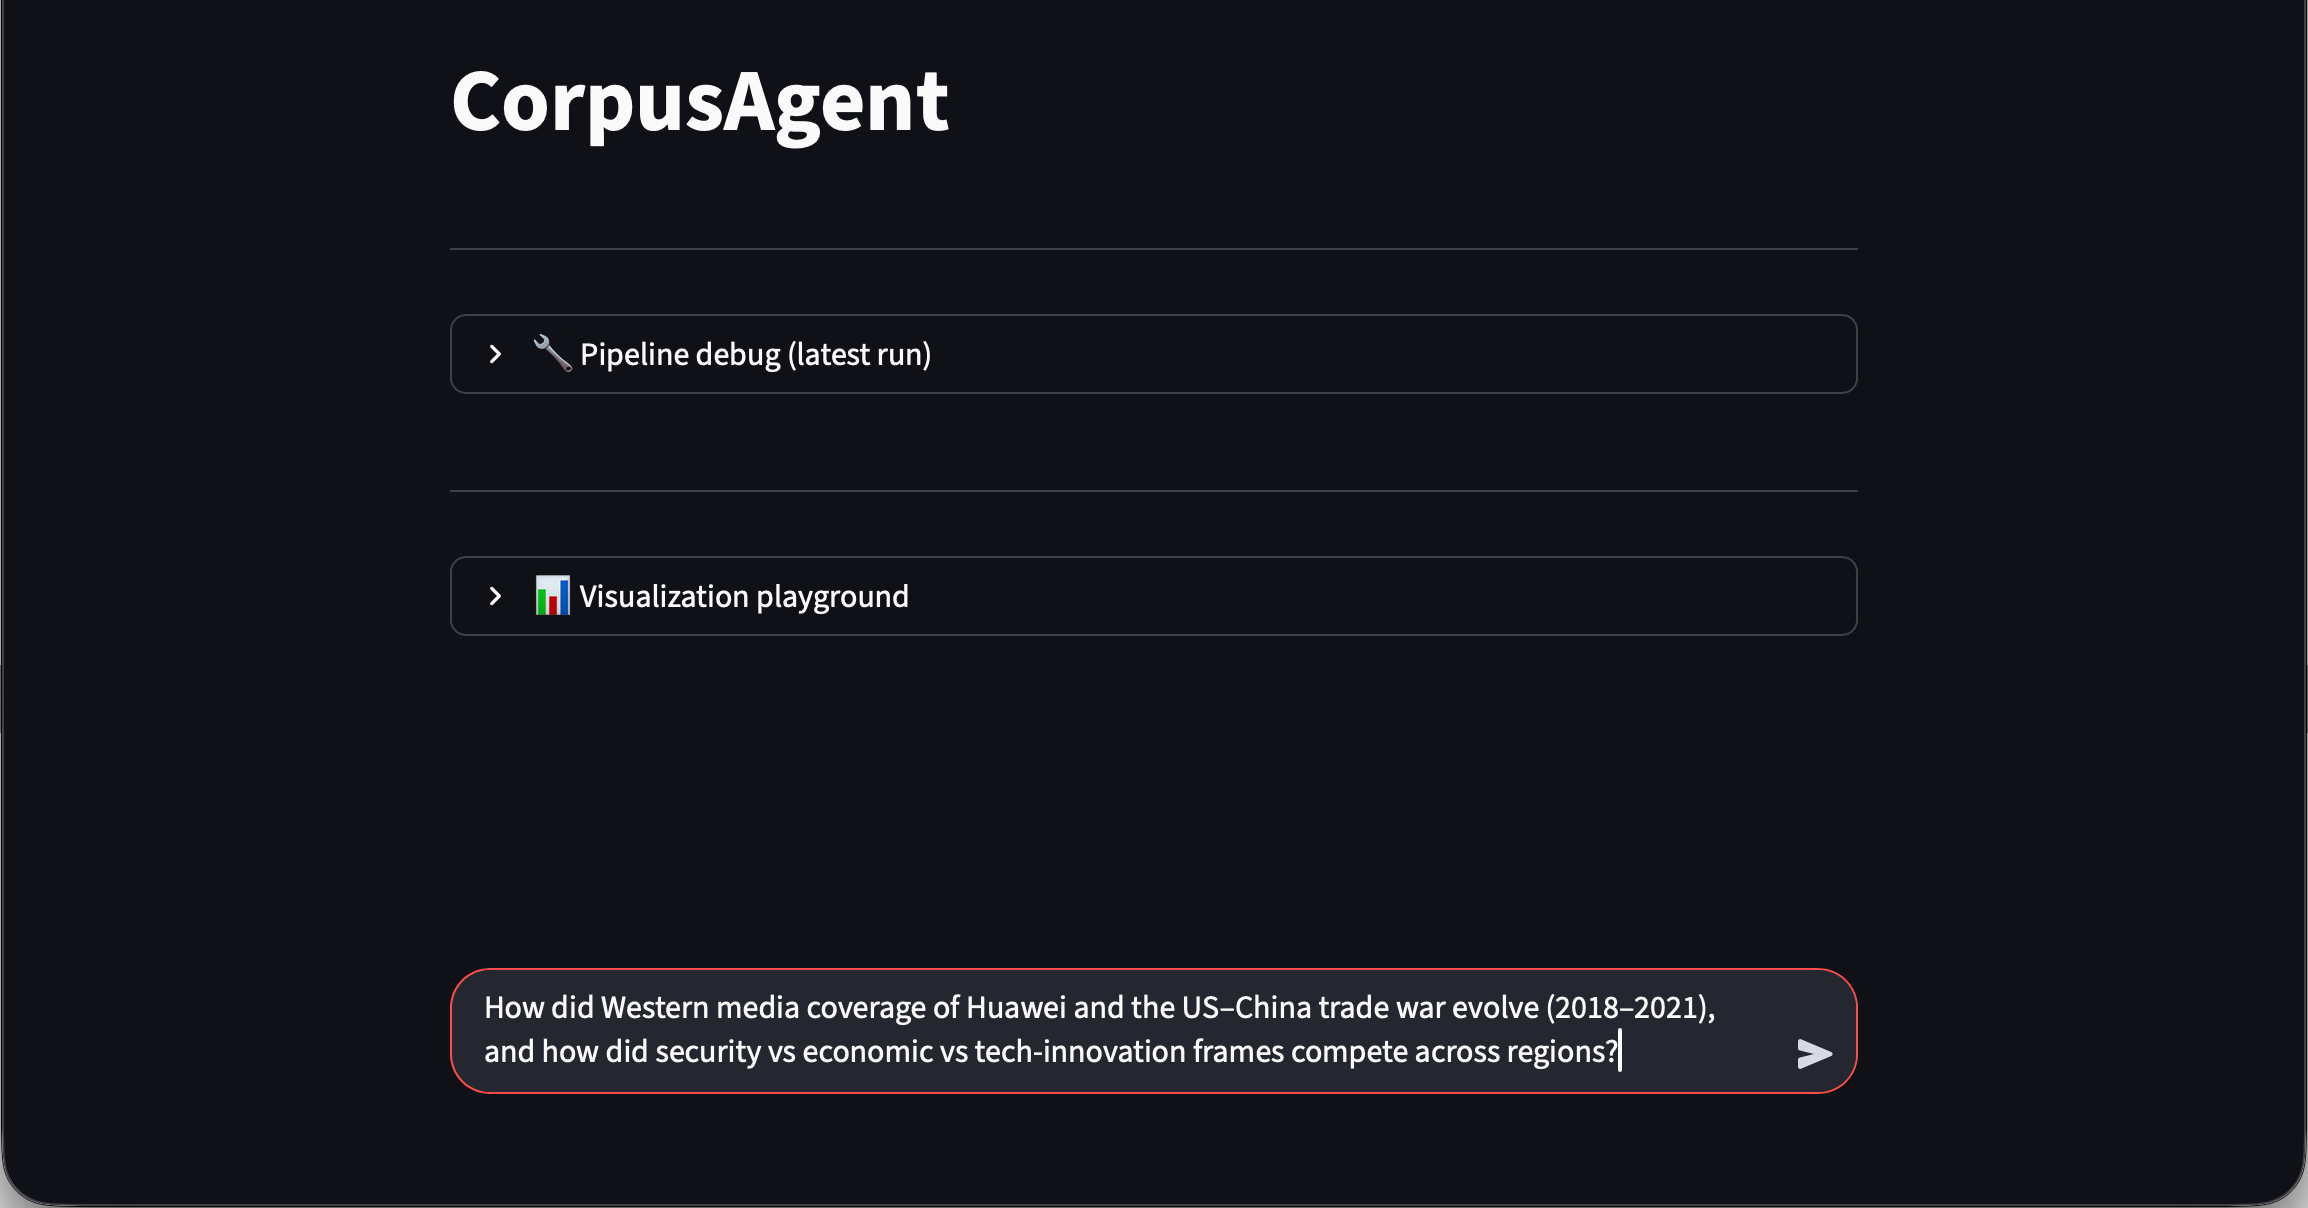
\includegraphics[width=0.95\textwidth]{Figures/walkthrough/ui_01_query_entry.png}
    \caption{CorpusAgent landing view with collapsible panels and query input field.}
    \label{fig:ui-query-entry}
\end{figure}

The application starts in a minimal state, exposing two collapsible system panels ("Pipeline debug" and "Visualization playground") and a persistent query input field (Figure~\ref{fig:ui-query-entry}). Submitting a query triggers the pipeline run, which then persists run metadata and intermediate artifacts for later inspection.

\section{Step 2 - Pipeline execution State}

\begin{figure}[ht]
    \centering
    
\includegraphics[width=0.95\textwidth]{Figures/walkthrough/ui_02_running_state.png}
    \caption{Query submitted; the system indicates an active run (retrieval + NLP execution).}
    \label{fig:ui-running}
\end{figure}

After submission, the UI transitions into a run state and displays an execution indicator (Figure~\ref{fig:ui-running}). Internally, this corresponds to the orchestration of retrieval and subsequent processing stages, as described in the section Pipeline orchestration \ref{PipelinePlanningLayer}.

\section{Step 3 - Final synthesized answer}

\begin{figure}[ht]
    \centering
    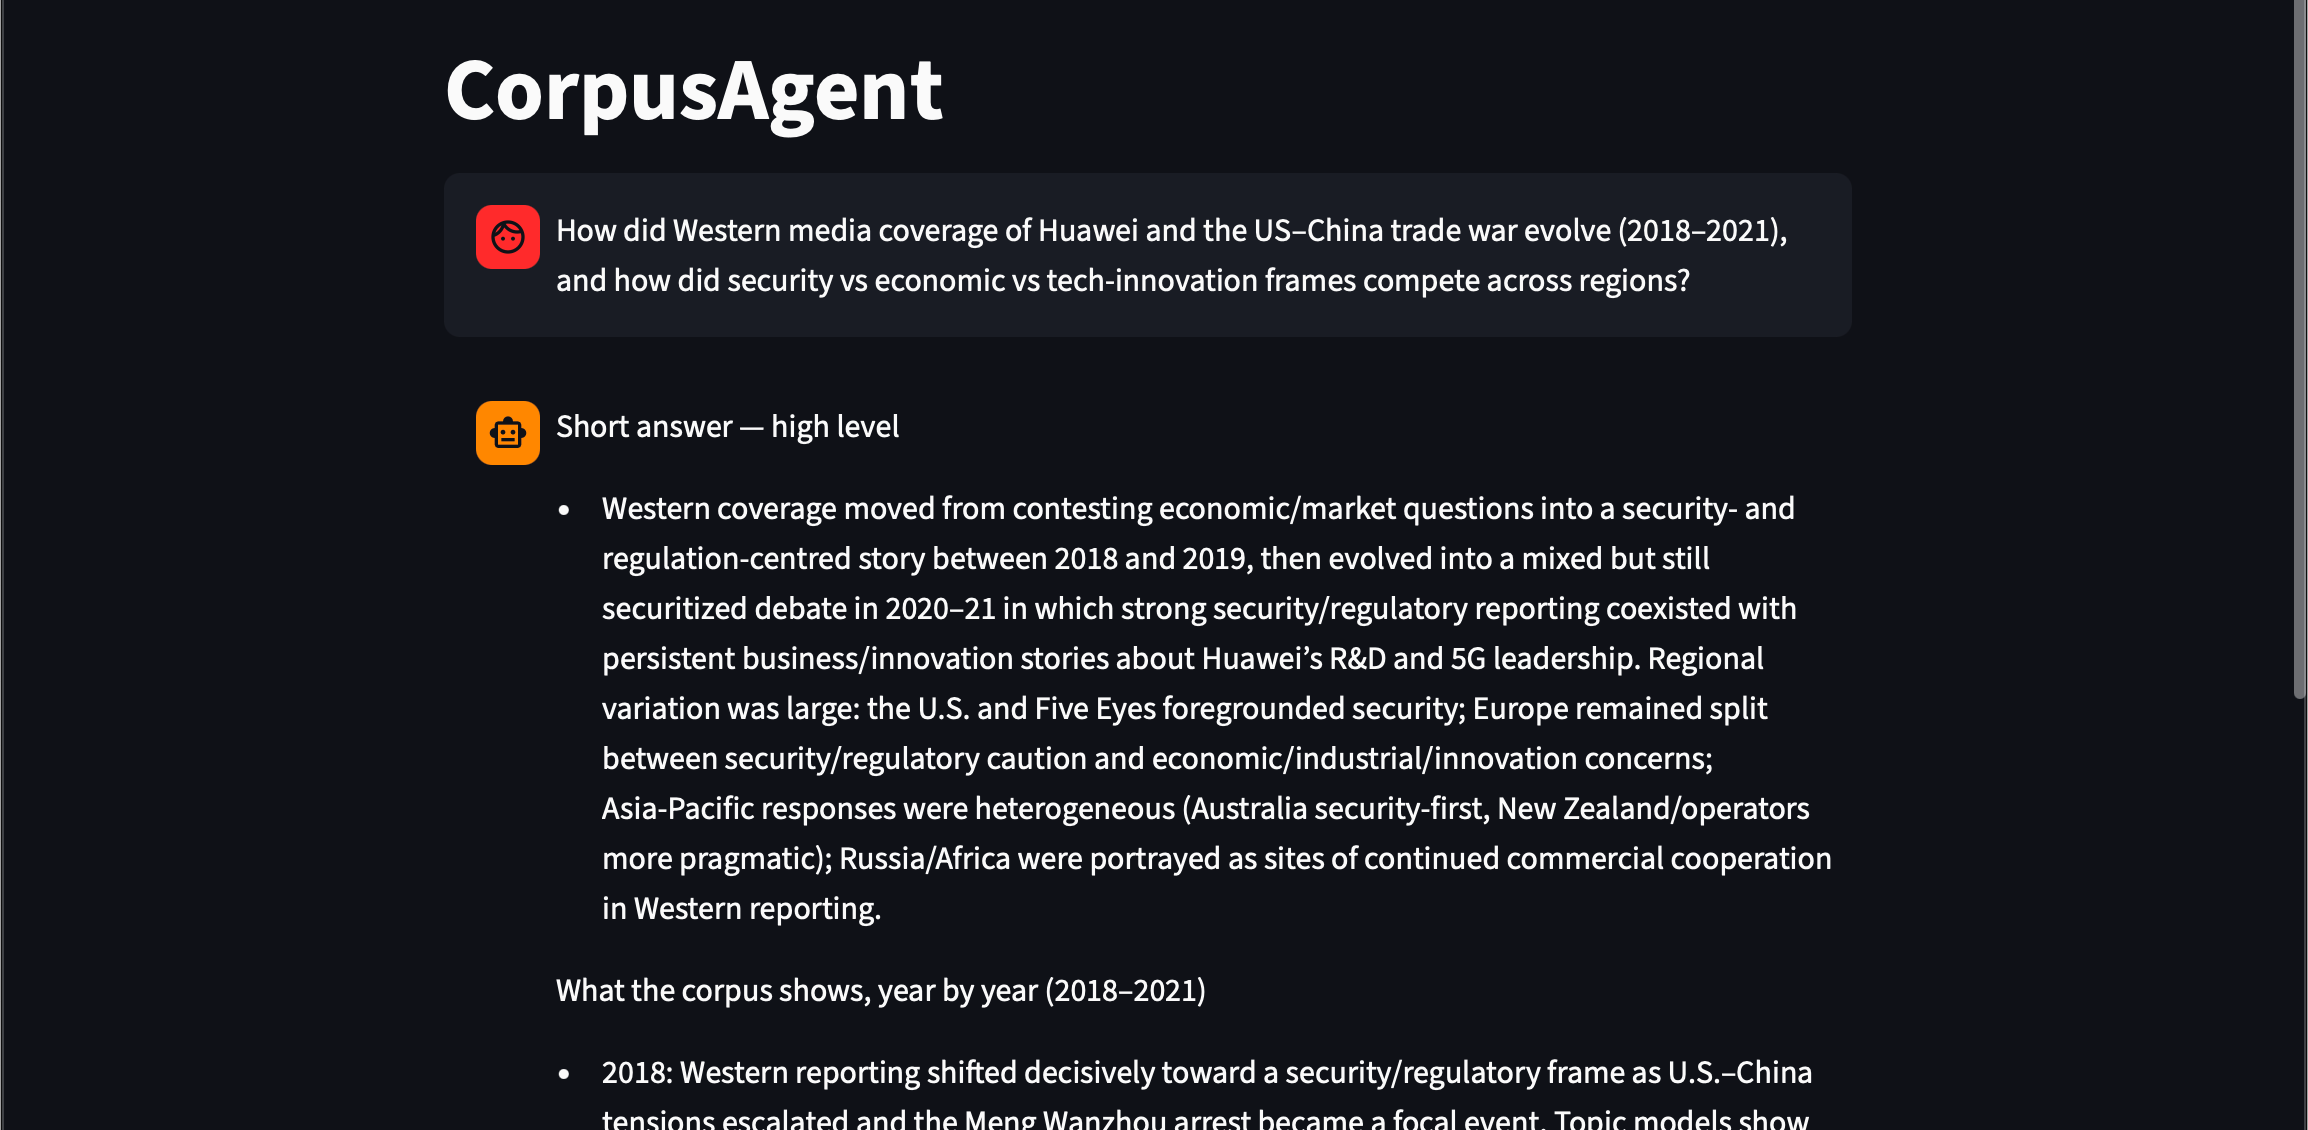
\includegraphics[width=0.95\textwidth]{Figures/walkthrough/ui_03_final_answer.png}
    \caption{Final synthesized answer displayed in the UI after pipeline completion.}
    \label{fig:ui-final-answer}
\end{figure}

Once the run completes, the final LLM-synthesized response is rendered in the chat view (Figure~\ref{fig:ui-final-answer}). This output corresponds to the terminal synthesis stage, where temporally aggregated evidence is transformed into a structured narrative answer.

\FloatBarrier

\section{Step 4 - Run introspection via "Pipeline debug"}

\begin{figure}[H]
    \centering
    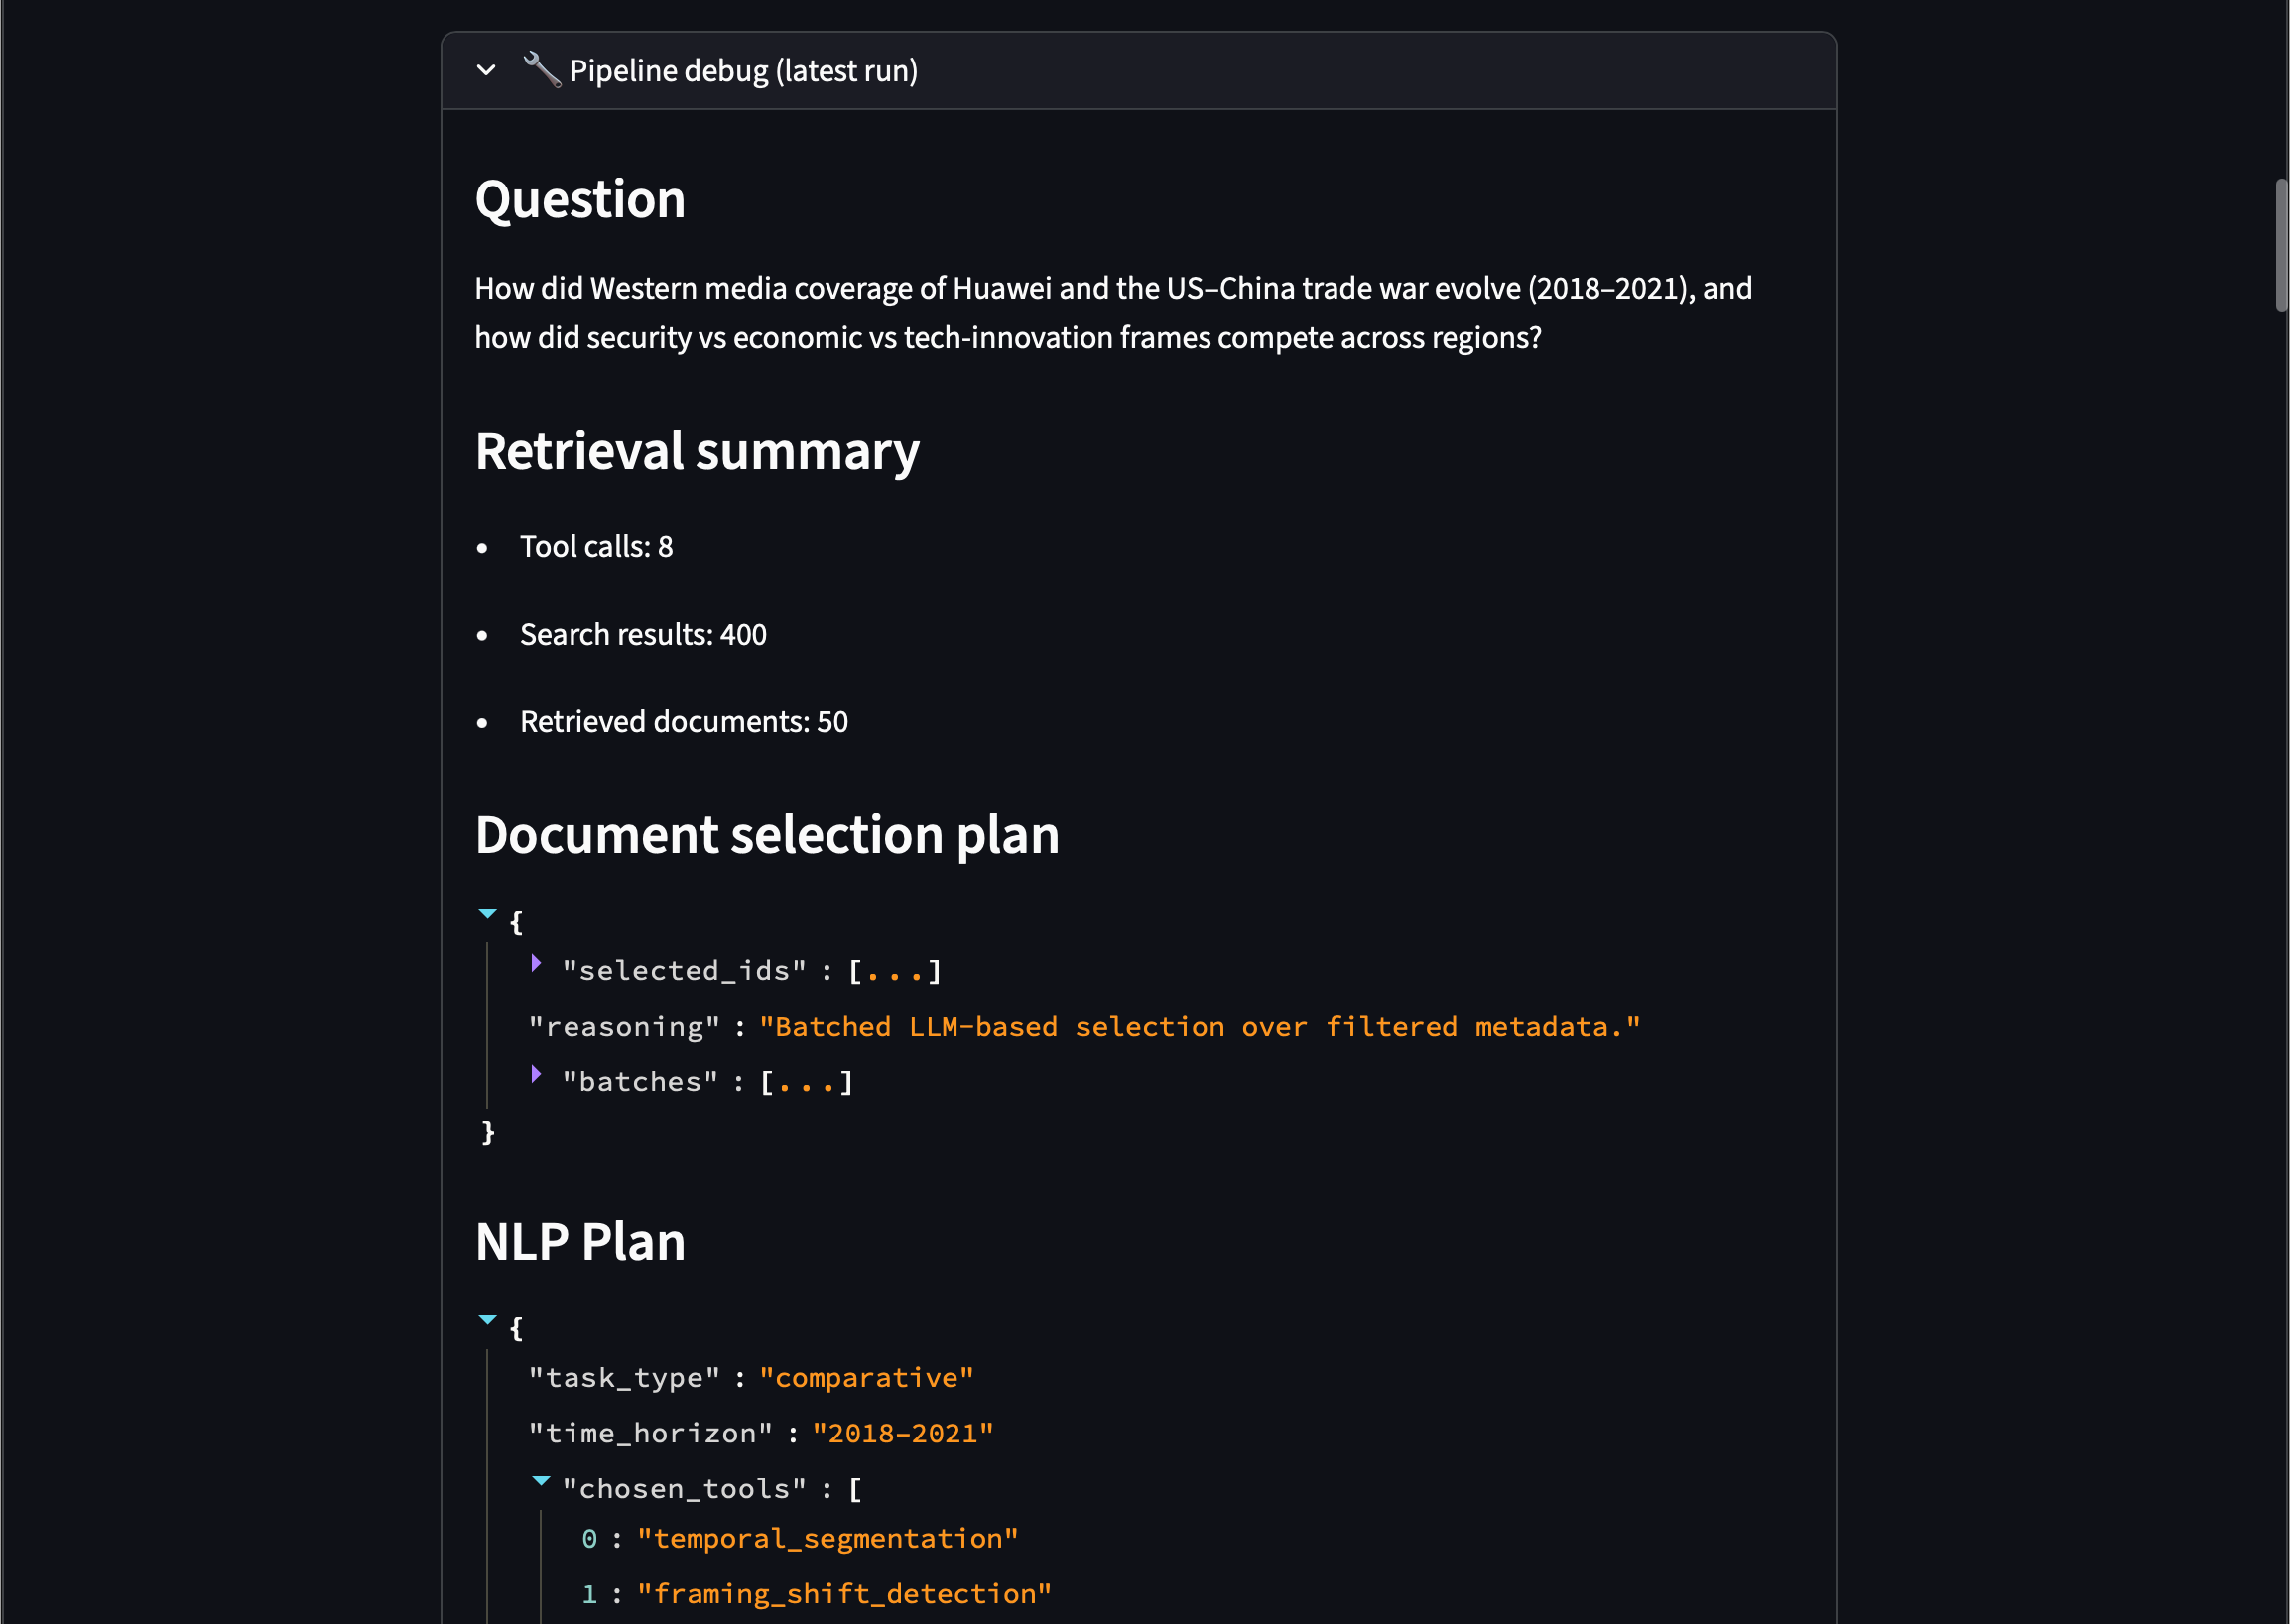
\includegraphics[width=0.95\textwidth]{Figures/walkthrough/ui_04_pipeline_debug.png}
    \caption{Expanded "Pipeline debug" panel showing detailed run metadata and intermediate artifacts.}
    \label{fig:ui-pipeline-debug}
\end{figure}

For transparency and debugging, the "Pipeline debug" panel exposes structured artifacts from the latest run (Figure~\ref{fig:ui-pipeline-debug}). This includes a compact retrieval summary (e.g., number of tool calls and retrieved documents), as well as JSON-based planning outputs such as the document selection plan and the NLP plan. These artifacts allow the run’s internal decision-making to be inspected independently of the final answer.

\FloatBarrier

\section{Step 5 - Accessing the Visualization Playground}

\begin{figure}[H]
    \centering
    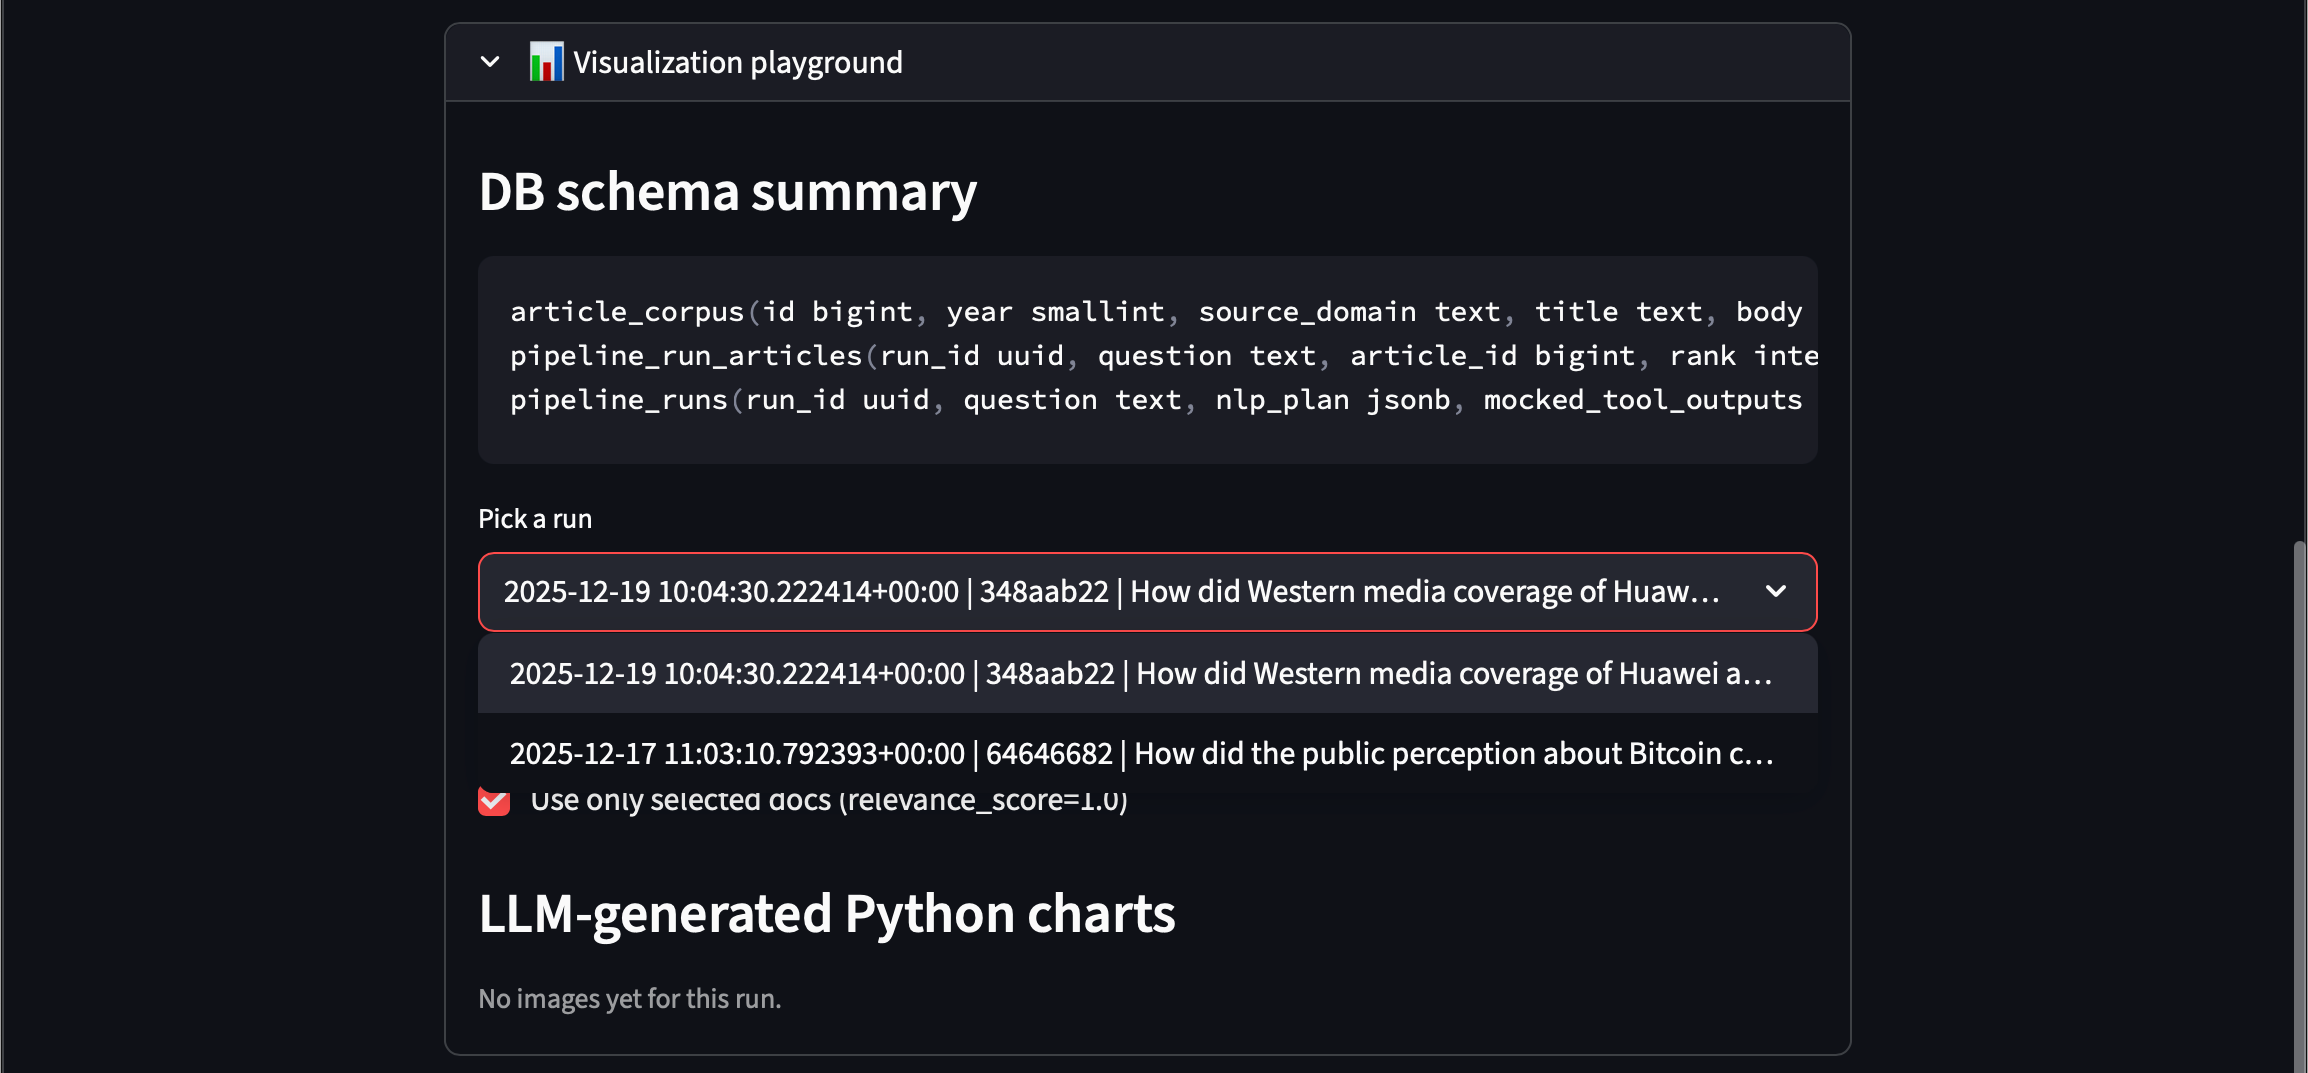
\includegraphics[width=0.95\textwidth]{Figures/walkthrough/ui_05_viz_playground_overview.png}
    \caption{Visualization Playground panel with schema summary and run selection.}
    \label{fig:ui-viz-playground}
\end{figure}

The "Visualization playground" is exposed as a separate panel that operates on stored run data (Figure~\ref{fig:ui-viz-playground}). The UI displays a condensed database schema summary and provides a dropdown to select a run. This design makes the visualization generation reproducible and run-centric: all charts are explicitly tied to a run\_id.

\FloatBarrier

\section{Step 6 - LLM-generated visualization plan (JSON)}

\begin{figure}[H]
    \centering
    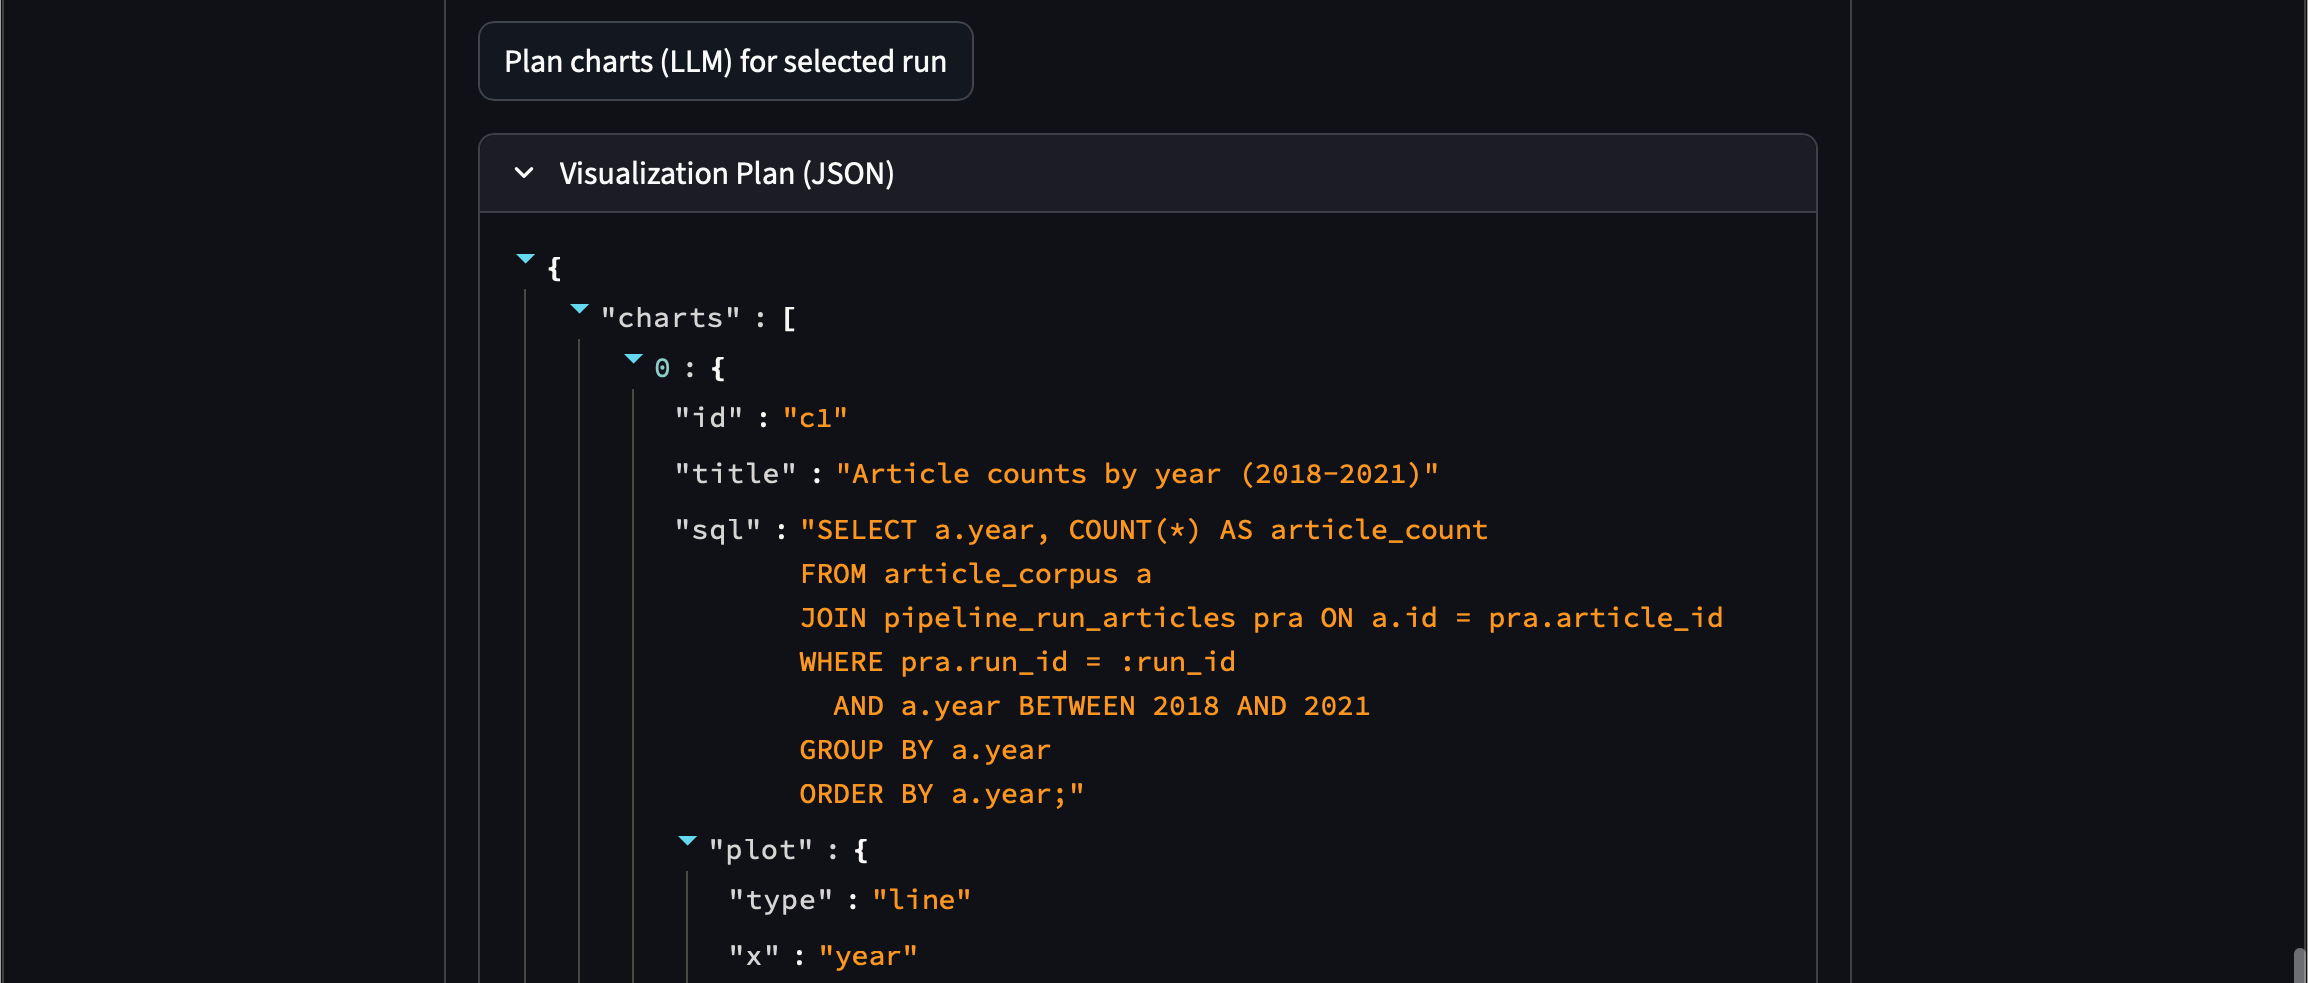
\includegraphics[width=0.95\textwidth]{Figures/walkthrough/ui_06_viz_plan_json.png}
    \caption{Visualization Plan in JSON form, including SQL queries and plot specifications.}
    \label{fig:ui-viz-plan}
\end{figure}

After selecting a run, the system generates a visualization plan (Figure~\ref{fig:ui-viz-plan}). The plan is represented as structured JSON containing (i) chart identifiers and titles, (ii) SQL queries scoped to the selected run\_id, and (iii) lightweight plot specifications (e.g., plot type and axis bindings). This plan serves as an intermediate, inspectable representation before any code is executed.

\FloatBarrier

\section{Step 7 - Generated plotting code (Python)}

\begin{figure}[H]
    \centering
    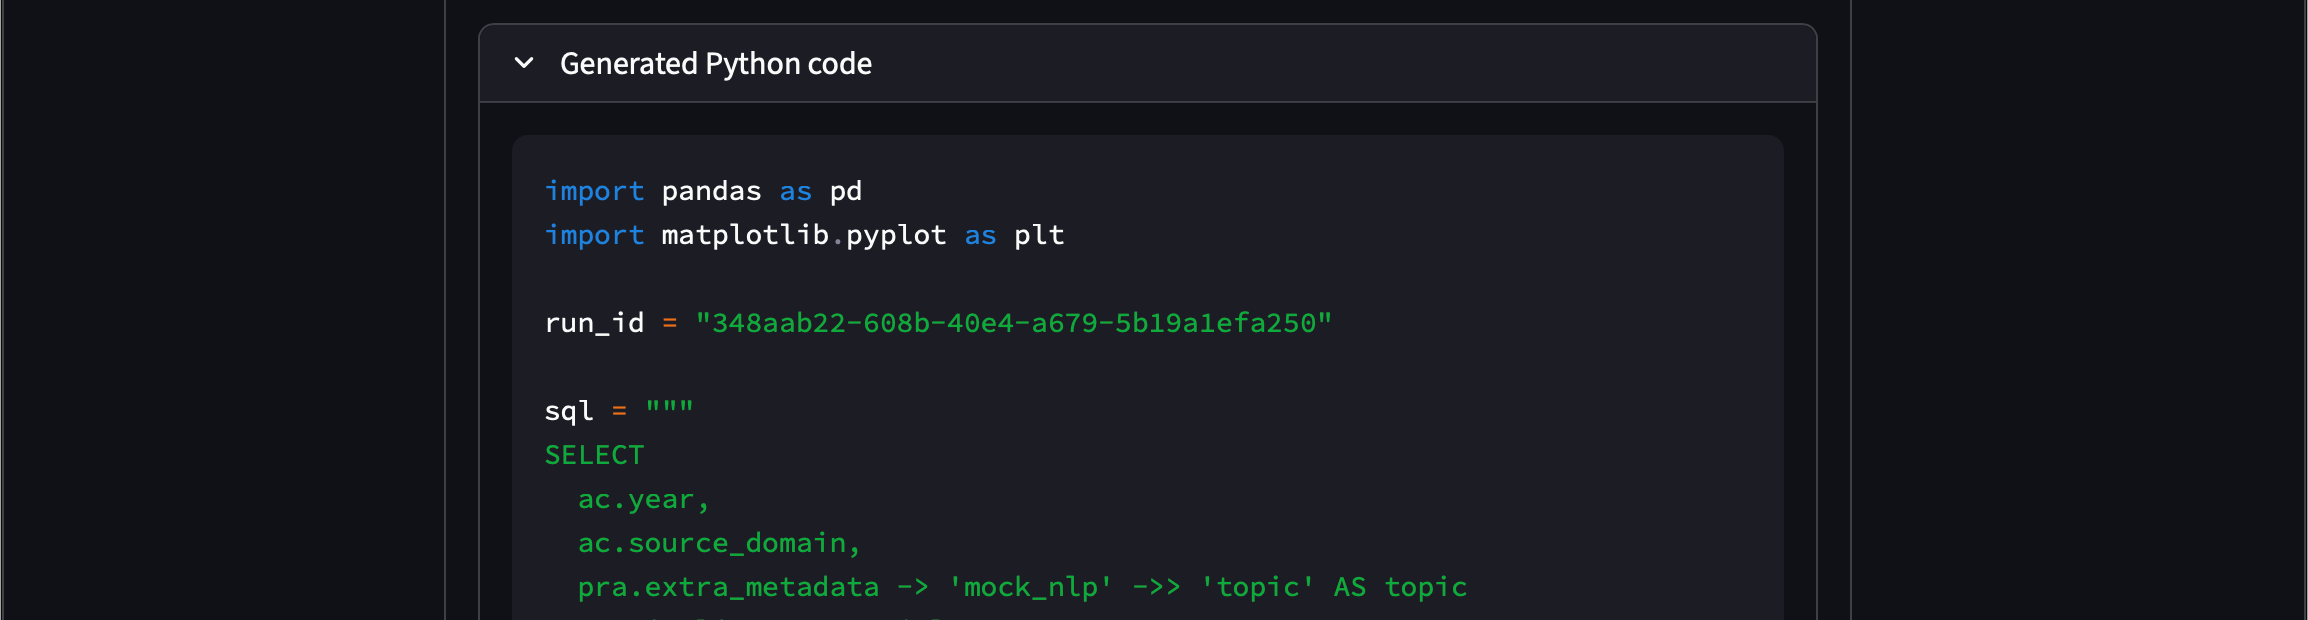
\includegraphics[width=0.95\textwidth]{Figures/walkthrough/ui_07_generated_code.png}
    \caption{LLM-generated Python code used to query the database and render charts.}
    \label{fig:ui-generated-code}
\end{figure}

Based on the JSON plan, the system generates executable Python code (Figure~\ref{fig:ui-generated-code}). The code queries the working dataset for the selected run, performs minimal transformations (e.g., normalizing labels into a small set of frames), and renders charts with Matplotlib. Persisting this code can be used for reproducibility and for diagnosing failures when chart generation does not succeed.

\FloatBarrier

\section{Step 8 - Chart rendering and output inspection}

\begin{figure}[H]
    \centering
    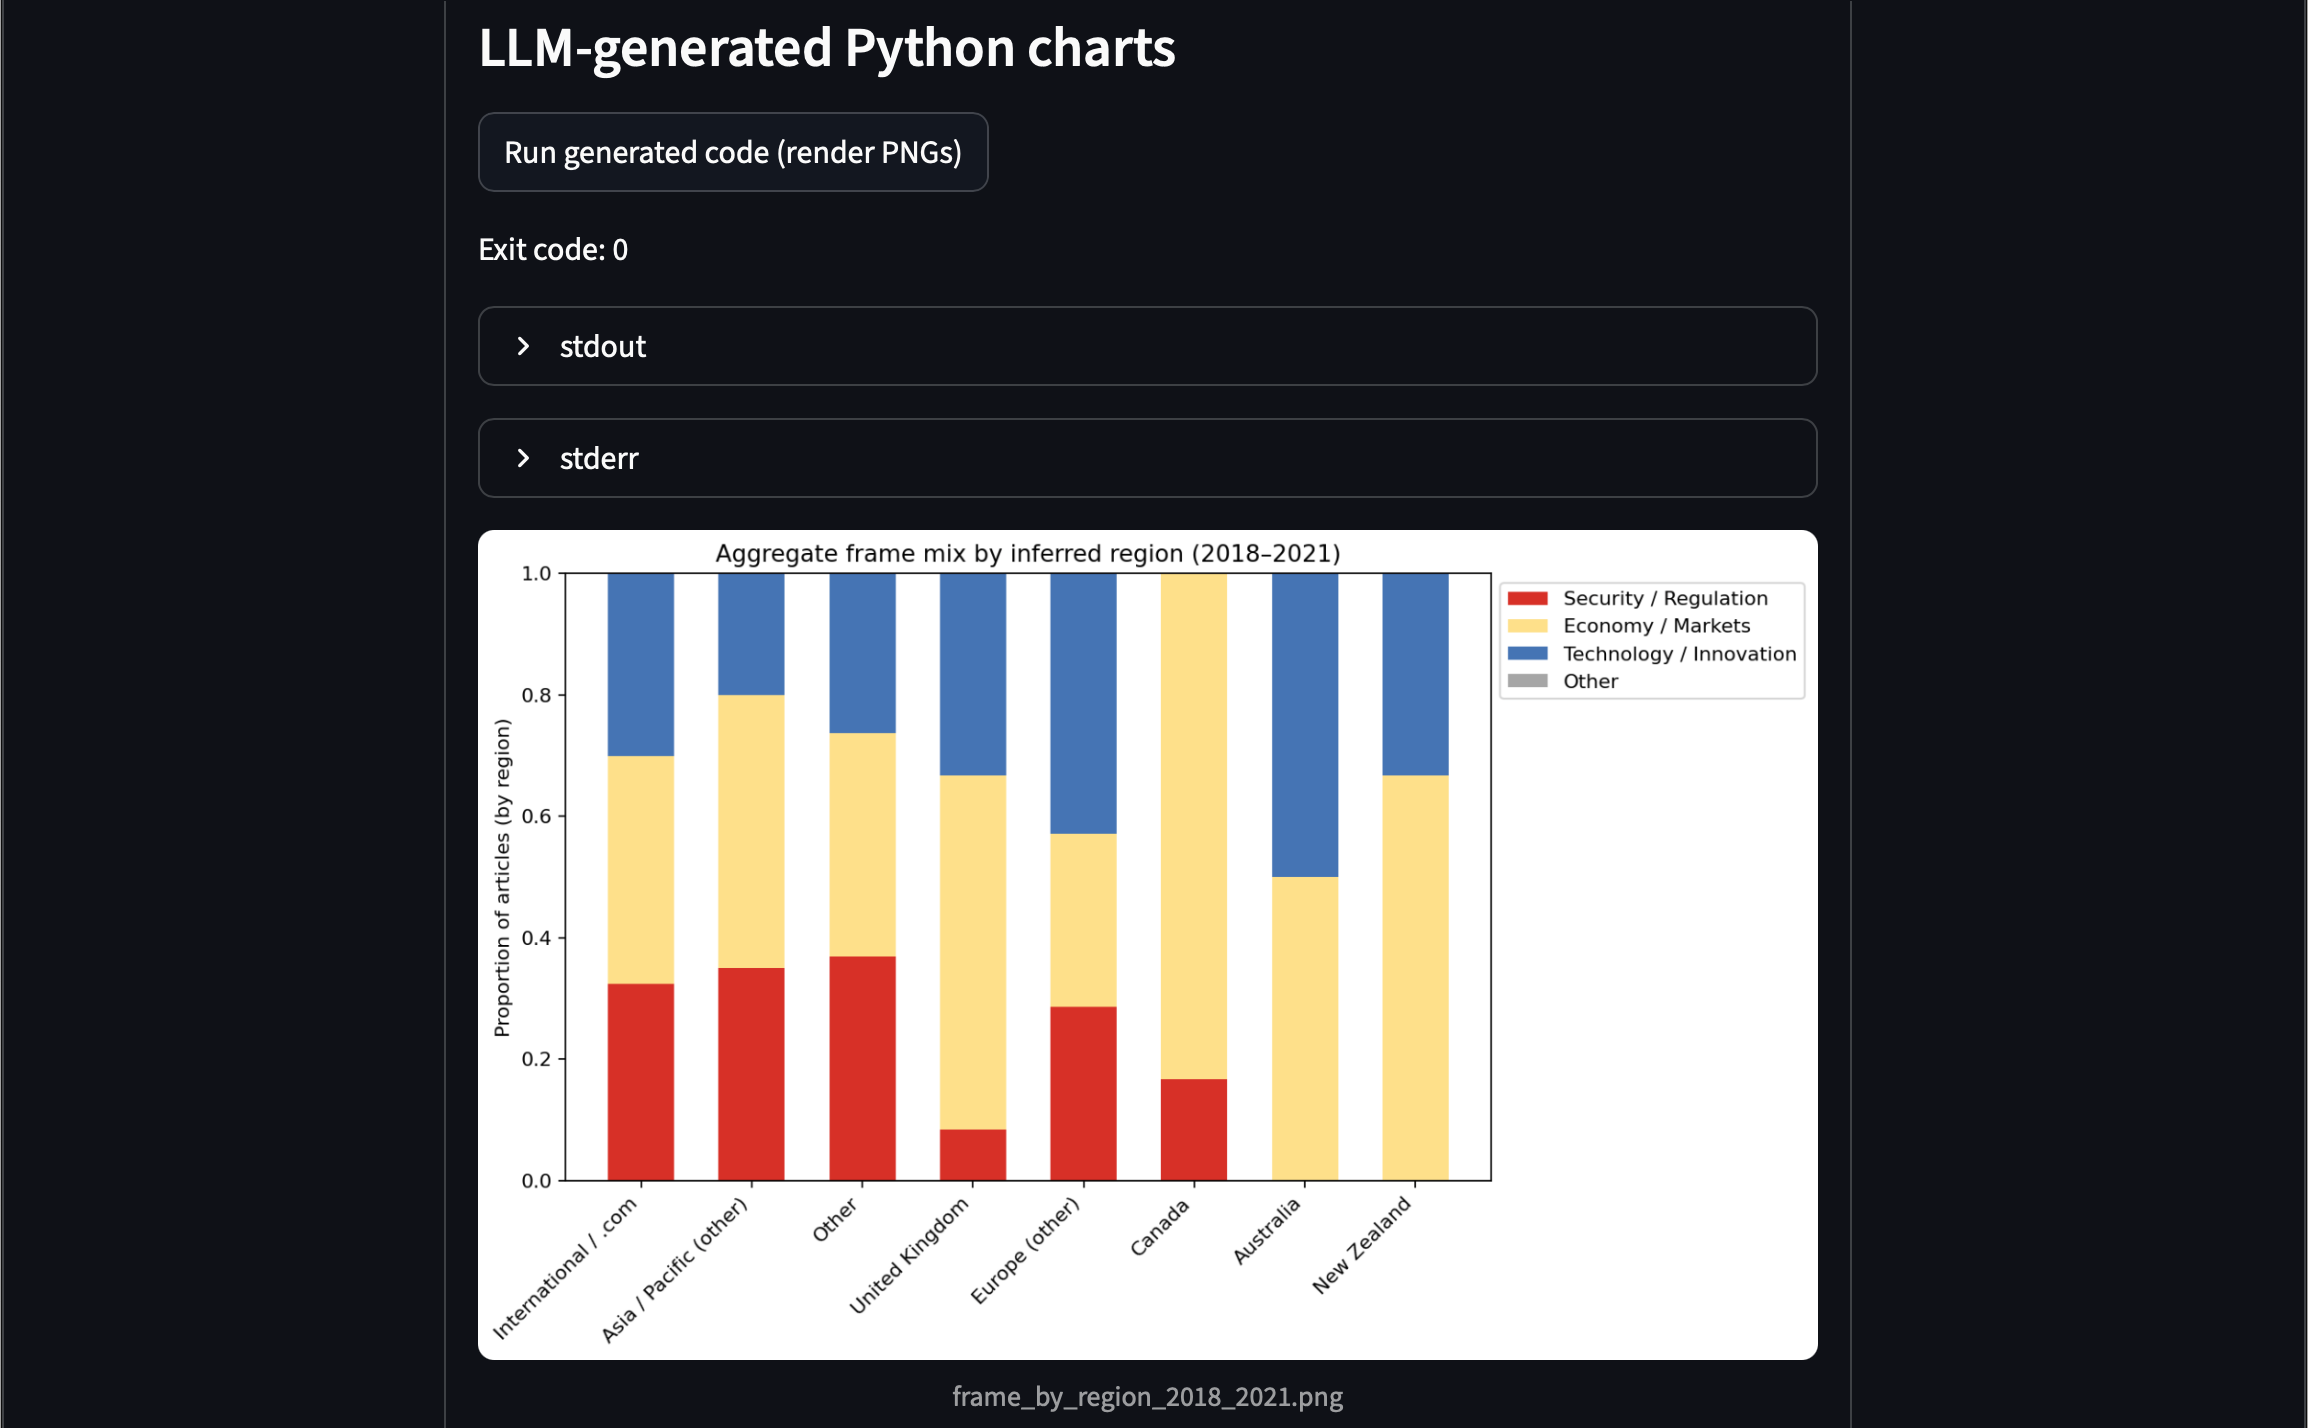
\includegraphics[width=0.95\textwidth]{Figures/walkthrough/ui_08_rendered_charts.png}
    \caption{Rendered charts displayed in the UI, including execution status and logs.}
    \label{fig:ui-rendered-charts}
\end{figure}

Executing the generated code produces PNG outputs, which are then displayed directly in the interface (Figure~\ref{fig:ui-rendered-charts}). The panel additionally exposes the process exit code as well as captured stdout/stderr, enabling a controlled debugging workflow. The resulting plots provide quantitative views (e.g., frame proportions over time or by inferred region) that complement the final answer.

\FloatBarrier

\section{Step 9 - Persisted artifacts on disk}

\begin{figure}[H]
    \centering
    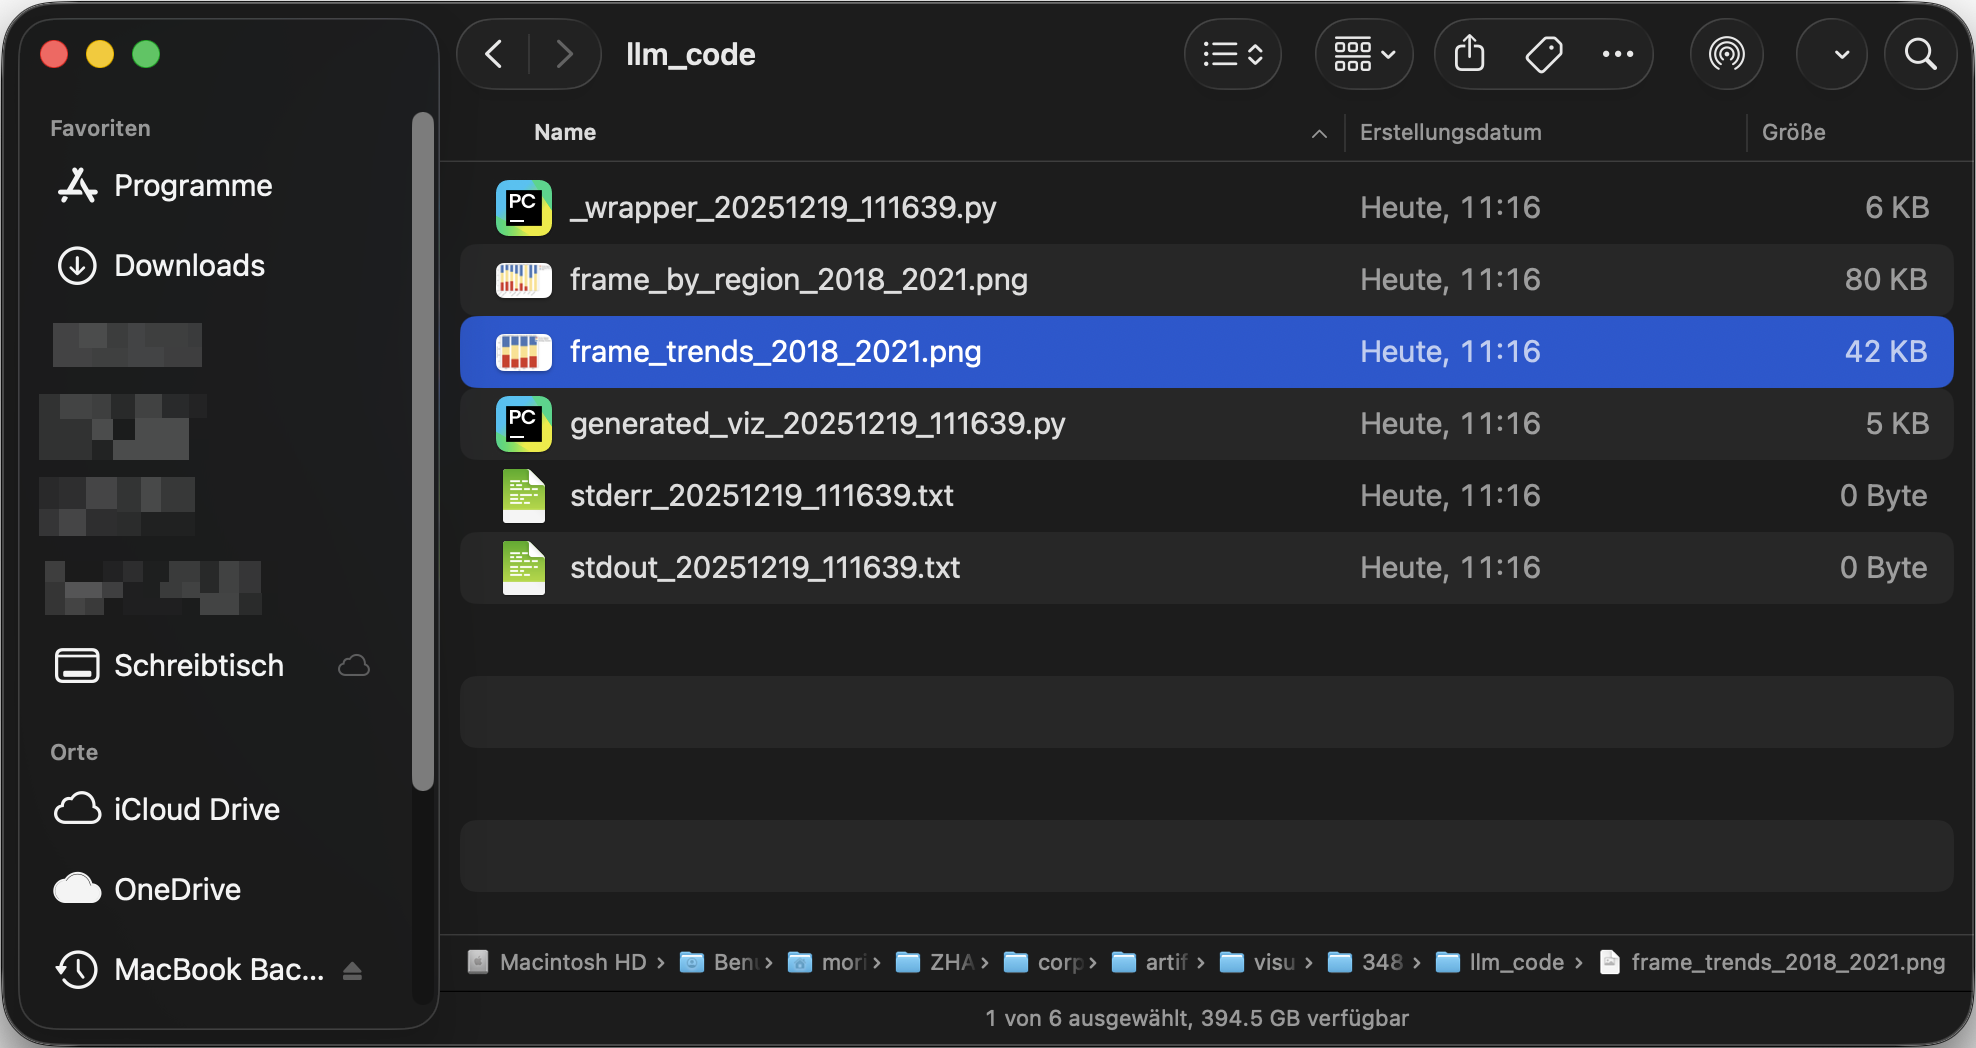
\includegraphics[width=0.95\textwidth]{Figures/walkthrough/ui_09_artifact_folder.png}
    \caption{Visualization artifacts persisted to disk (generated code, wrapper, logs, PNG outputs).}
    \label{fig:ui-artifacts}
\end{figure}

Finally, the visualization pipeline persists all outputs for the run to disk (Figure~\ref{fig:ui-artifacts}). The artifact directory contains the generated plotting script, an execution wrapper, stdout/stderr logs, and the produced PNG files. This persistence supports reproducibility, post-hoc inspection, and iterative refinement of visualization prompts and constraints.



% Indicate the main file. Must go at the beginning of the file.
% !TEX root = ../main.tex

%----------------------------------------------------------------------------------------
% CHAPTER TEMPLATE
%----------------------------------------------------------------------------------------


\chapter{Results} % Main chapter title

\label{ChapterResults} % Change X to a consecutive number; for referencing this chapter elsewhere, use \ref{ChapterX}

%----------------------------------------------------------------------------------------
% SECTION 1
%----------------------------------------------------------------------------------------

\section{Experimental Setup}

All experiments were conducted on a 10\% subset of the CC-News corpus spanning 2016–2021. Media sentiment and topic trends were aggregated at the yearly level unless stated otherwise. The system automatically generated analytical plans, selected NLP tools, executed the analyses, and produced visualizations for each question. Selected figures are shown to support the qualitative interpretation of results.

The analytical pipeline relies on a set of modular NLP tools that are invoked dynamically by the LLM during execution. For the purpose of this thesis, the tools were implemented with mocked outputs to demonstrate the system architecture, planning behavior, and result integration without relying on fully operational external services. Each tool represents a distinct analytical capability commonly used in large-scale text analysis.

\subsection{NLP Analysis Tools}

The following NLP tools were available to the system during execution. All tools were implemented with mocked outputs for demonstration and evaluation purposes:

\begin{itemize}
    \item \texttt{sentiment\_over\_time}: Computes aggregated sentiment trends across time intervals.
    \item \texttt{volatility\_of\_sentiment}: Measures temporal fluctuations in sentiment intensity.
    \item \texttt{emotion\_distribution\_over\_time}: Tracks the distribution of emotional categories over time.
    \item \texttt{topic\_trend\_over\_time}: Identifies and tracks dominant topics across temporal segments.
    \item \texttt{dynamic\_topic\_shift\_detection}: Detects significant changes in topic prevalence.
    \item \texttt{event\_detection}: Identifies temporally localized events reflected in the corpus.
    \item \texttt{burst\_detection}: Detects sudden increases in coverage or term usage.
    \item \texttt{named\_entity\_trend\_tracking}: Tracks the temporal prominence of named entities.
    \item \texttt{relationship\_graph\_extraction}: Extracts co-occurrence graphs between entities.
    \item \texttt{framing\_shift\_detection}: Identifies changes in narrative framing over time.
    \item \texttt{stance\_detection\_over\_time}: Tracks changes in expressed stance toward entities or topics.
    \item \texttt{salient\_quote\_extraction}: Extracts representative or influential quotations.
    \item \texttt{fact\_density\_estimation}: Estimates the ratio of factual statements within documents.
    \item \texttt{source\_bias\_comparison}: Compares sentiment and framing across sources.
    \item \texttt{temporal\_segmentation}: Segments the corpus into meaningful temporal phases.
    \item \texttt{document\_clustering}: Groups documents based on semantic similarity.
    \item \texttt{keyphrase\_evolution\_tracking}: Tracks the emergence and decline of keyphrases.
    \item \texttt{anomaly\_etection\_in\_discourse}: Identifies atypical discourse patterns.
    \item \texttt{confidence\_scoring\_of\_results}: Estimates confidence scores for aggregated findings.
\end{itemize}


\section{Core longitudinal Questions}

\subsection{Media Sentiment towards Donald Trump and Market Volatility}

\paragraph{User Query}

\textit{"How did media sentiment towards Donald Trump evolve from the 2016 campaign through his presidency, and how did these sentiment patterns relate to periods of heightened US equity-market volatility?"}

\paragraph{Research Question}

This analysis examines how media sentiment toward Donald Trump evolved from the 2016 campaign through his presidency (2016–2020), and how these sentiment patterns related to periods of heightened US equity-market volatility.

\paragraph{System-Generated Summary}
The system produced the following condensed answer based on the retrieved corpus and analytical outputs:

\begin{quote}
Media sentiment toward Donald Trump across 2016–2020 was predominantly negative overall but fluctuated year-to-year, with clear bursts of coverage each year 2017–2020. Measured yearly average sentiment in the supplied analytics: 2016 (strongly negative), 2017 (negative), 2018 (an outlier positive mean in the series), 2019 (strongly negative), 2020 (negative). Sentiment volatility was high (avg change ~0.75) and the analytics flag strong bursts in 2017–2020.

The qualitative reporting links those sentiment shifts to equity-market volatility in a patterned way: sometimes media negativity coincided with elevated market fear (2018 tariffs, 2019 trade-tweet episodes, 2020 COVID sell-off and election jitters), but other periods showed a disconnect (2017: negative political coverage while major indices pushed to new highs and the VIX stayed low).
\end{quote}

\paragraph{Analytical Results}

Media sentiment toward Donald Trump was predominantly negative throughout the period 2016–2020, with substantial year-to-year variation. Sentiment was strongly negative in 2016 and 2017, shifted to a positive annual mean in 2018, and returned to strongly negative levels in 2019 before moderating slightly in 2020. Across all years, sentiment volatility was high and burst detection identified pronounced spikes in coverage between 2017 and 2020.

\paragraph{Relationship to Market Volatility}

Periods of heightened negative or uncertain media coverage sometimes coincided with elevated equity-market volatility. Notable alignments appear during the 2018 trade-policy escalations, repeated trade-related announcements in 2019, and the COVID-19 market shock in 2020. In these periods, coverage explicitly framed political decisions as market-relevant risk factors.

However, the relationship was not uniform. In 2017, negative political coverage coexisted with relatively subdued realized market volatility, suggesting a disconnect between political sentiment and immediate equity-market reactions. This indicates that negative media sentiment does not consistently translate into realized volatility and that market responses depend on the perceived economic relevance of events.

\begin{figure}[h]
    \centering
    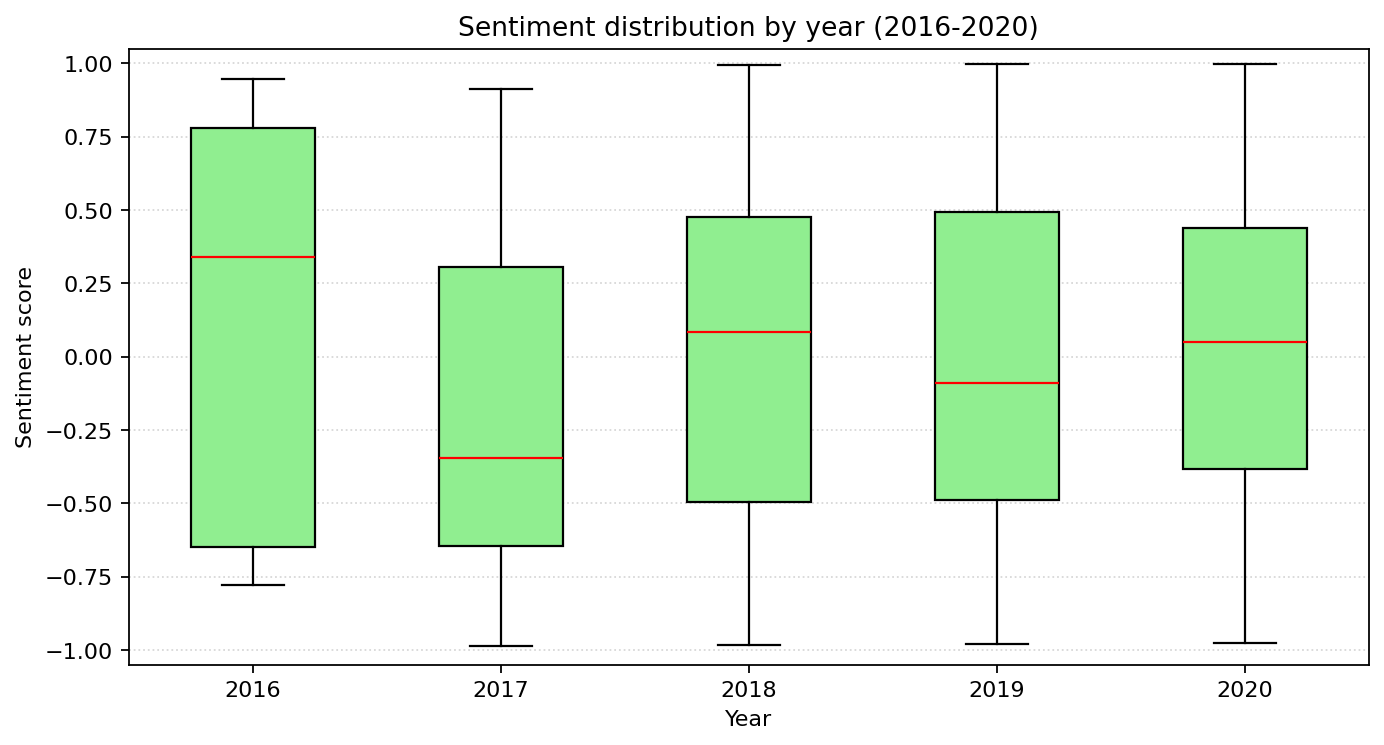
\includegraphics[width=0.8\textwidth]{Figures/sentiment_boxplot_by_year_a1_question.png}
    \caption{Media Sentiment toward Donald Trump (2016–2020) and US Equity-Market Volatility}
    \label{fig:media_sentiment_trump_market_volatility}
\end{figure}

\begin{figure}[h]
    \centering
    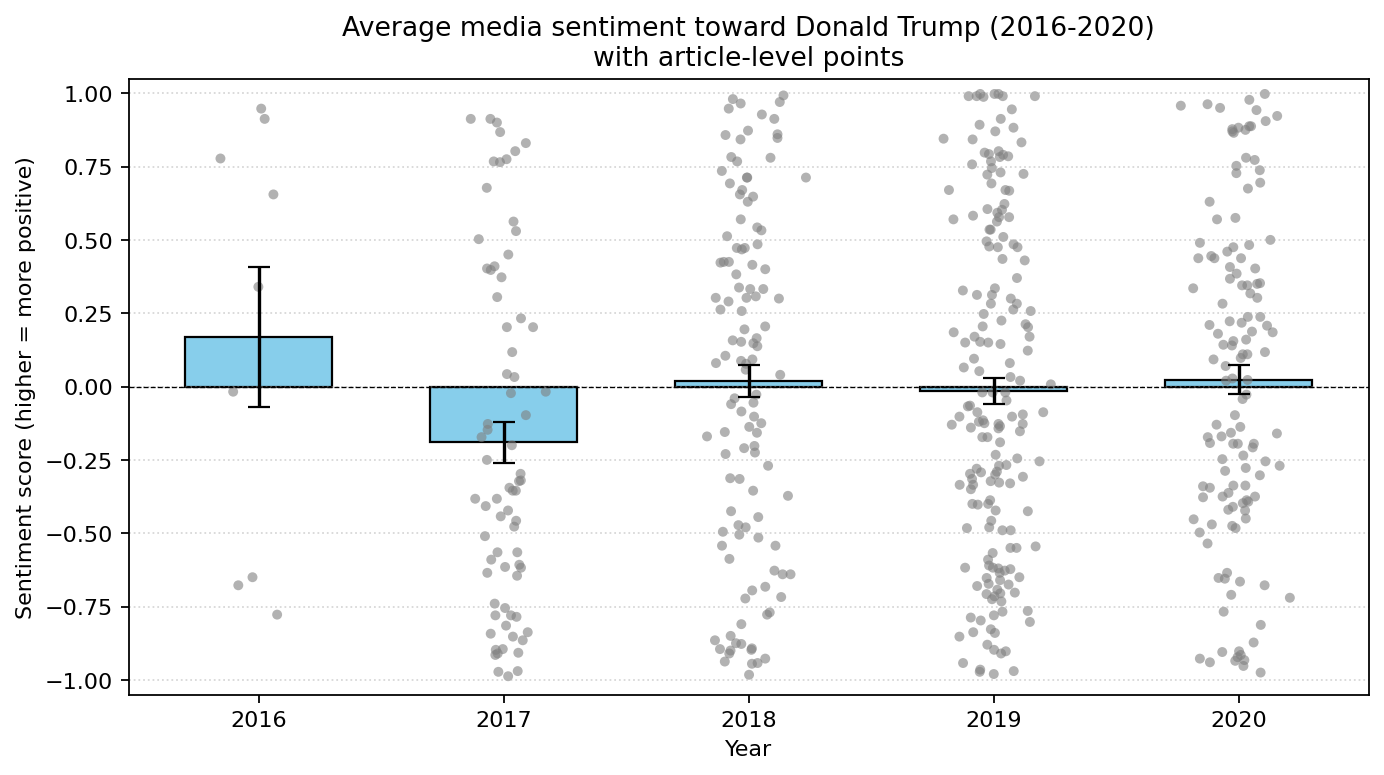
\includegraphics[width=0.8\textwidth]{Figures/sentiment_mean_by_year_a1_question.png}
    \caption{Mean Media Sentiment toward Donald Trump (2016–2020) and US Equity-Market Volatility}
    \label{fig:media_sentiment_trump_market_volatility_mean}
\end{figure}

\begin{figure}[h]
    \centering
    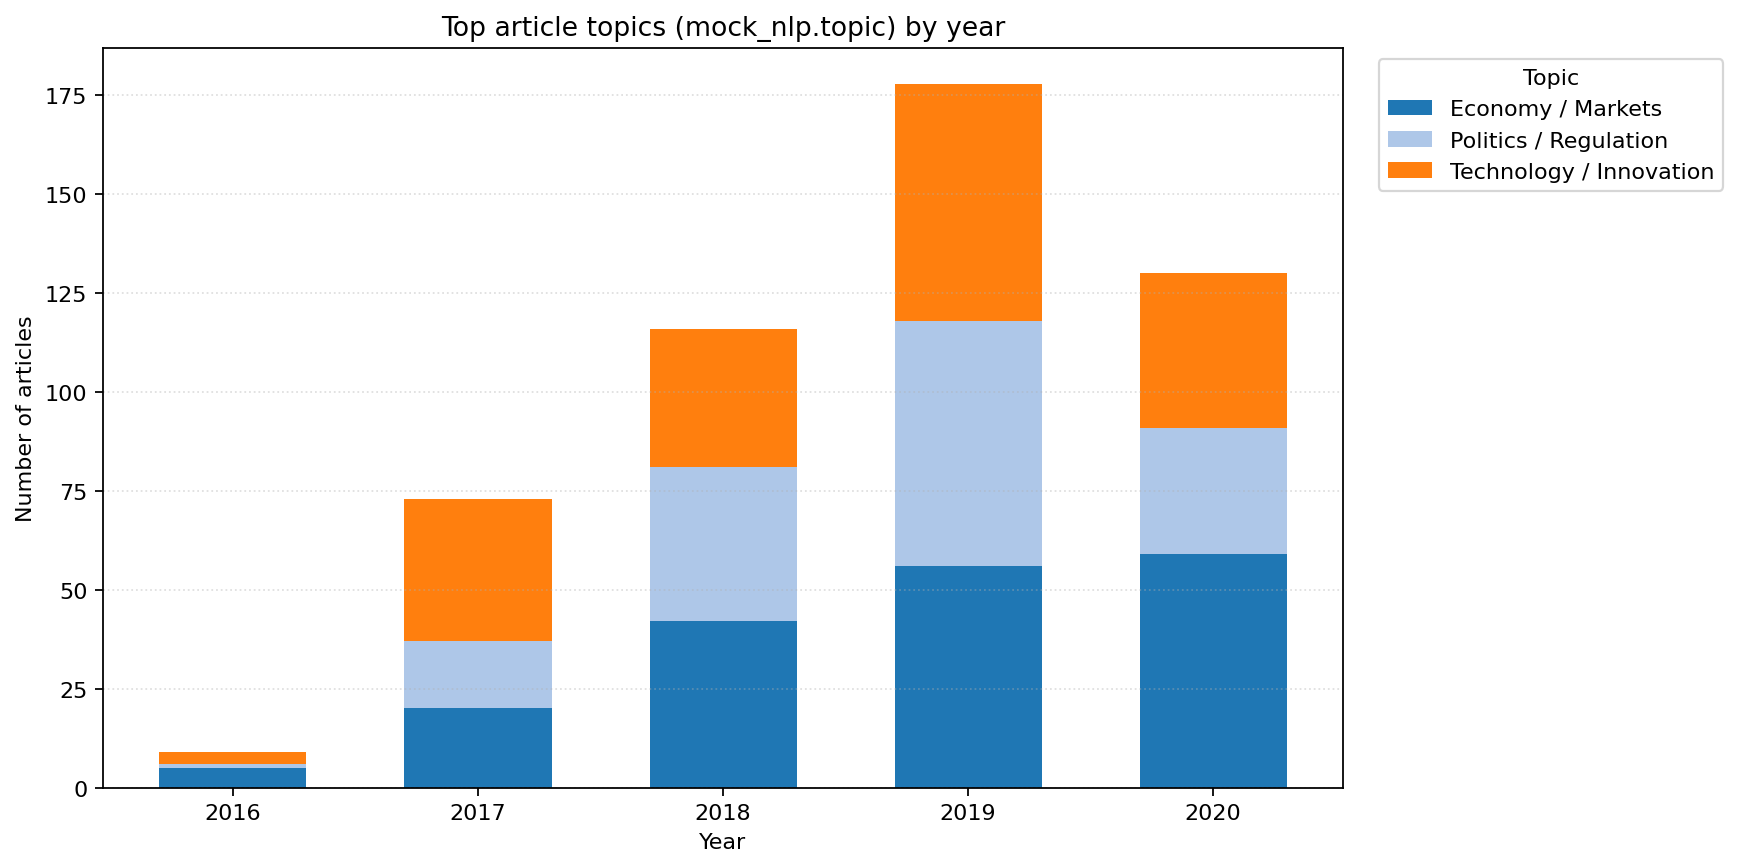
\includegraphics[width=0.8\textwidth]{Figures/topic_counts_by_year_a1_question.png}
    \caption{Topic Counts Related to Donald Trump (2016–2020)}
    \label{fig:topic_counts_trump}
\end{figure}


\paragraph{Summary}

In summary, media sentiment toward Donald Trump was consistently volatile and largely negative across his presidency, but its alignment with equity-market volatility was episodic rather than systematic. Media sentiment and market volatility aligned most clearly during periods where political events had direct economic implications, while purely political controversies often showed weaker or no immediate market response.
 

%------ Table of Figures, Tables, and Listings ------
\cleardoublepage
\phantomsection
\addcontentsline{toc}{chapter}{List of Figures}
\listoffigures
\cleardoublepage
\phantomsection
\addcontentsline{toc}{chapter}{List of Tables}
\listoftables
\cleardoublepage
\phantomsection
\addcontentsline{toc}{chapter}{List of Listings}
\lstlistoflistings
%-----------------------------------------------------

%----------------------------------------------------------------------------------------
% THESIS CONTENT - APPENDICES
%----------------------------------------------------------------------------------------
\appendix % Cue to tell LaTeX that the following "chapters" are Appendices

% Include the appendices of the thesis as separate files from the Appendices folder
% Uncomment the lines as you write the Appendices
% !TEX root = ../main.tex

%----------------------------------------------------------------------------------------
% APPENDIX A
%----------------------------------------------------------------------------------------

\chapter{Detailed CorpusAgent Trace Example}

\section{CorpusAgent Trace: Facebook / Cambridge Analytica (2016--2019)}
\label{app:trace-facebook-cambridge}

\subsection{Question and System Answer}
\begin{tcolorbox}
\textbf{User Question:} \\
How did Facebook coverage shift from innovation/growth framing to privacy/regulation framing around the Cambridge Analytica scandal (2016--2019), and how did this correspond to FB stock drawdowns?
\end{tcolorbox}

\begin{tcolorbox}
\textbf{System Answer (condensed):}

\textbf{Short answer.} Media framing moved from an innovation/growth emphasis toward a dominant privacy/regulation frame centered on Cambridge Analytica between 2017--2019, with the pivot concentrated in 2018 when the Cambridge Analytica revelations produced large spikes in Facebook/``Cambridge'' mentions and regulatory/legal language. That framing shift coincided with major market reactions: the provided context reports an immediate one-day, multi-billion-dollar market loss when the revelations broke in 2018 and a much larger late-July 2018 selloff (reported as roughly a 20\% wipeout) when growth metrics softened and regulatory risk looked more consequential. In 2019 continuing regulatory headlines (FTC accrual/settlement, fines) are linked to another very large one-day market-value hit mid-year and only modest rebounds on settlement approval.

\vspace{0.5em}
\textbf{Evidence from the provided analytics.}
\begin{itemize}
    \item \textbf{Framing:} 2016--2017 coverage was more mixed/anticipatory (GDPR-driven regulatory discussion described as cautionary rather than scandal-driven). In 2018 ethics/regulation and risk/crisis frames rise (ethics/regulation $\approx 0.54$, risk/crisis $\approx 0.31$), and 2019 keeps ethics/regulation elevated (ethics/regulation $\approx 0.445$).
    \item \textbf{Keyphrases \& entities:} ``Cambridge'' and ``Analytica'' spike in 2018 (Cambridge: 0 in 2017 $\rightarrow$ 18 in 2018; Analytica: 0 $\rightarrow$ 13). ``Facebook'' mentions also jump (4 $\rightarrow$ 56). Privacy-related keyphrase weight increases into 2019.
    \item \textbf{Topics:} Topic trends shift toward Politics/Regulation dominance in 2018--2019, while Technology/Innovation becomes less prominent relative to earlier years.
    \item \textbf{Market correspondence (reported in summaries):} The context links major drawdowns to (i) the initial 2018 revelations and (ii) later 2018 growth concerns under heightened regulatory risk, with additional 2019 drawdowns tied to regulatory developments.
\end{itemize}

\vspace{0.5em}
\textbf{Limitations.} The context provides year-level analytics and narrative summaries but no daily price/return series and no automated drawdown-alignment tool. Therefore, precise event-study abnormal returns, lead--lag correlations, and time-aligned plots cannot be computed from the provided material alone.

\vspace{0.5em}
\textbf{Needed for tighter quantitative alignment.}
\begin{itemize}
    \item FB price/volume series (daily or higher-frequency) for 2016--2019,
    \item timestamps or daily counts for media spikes (e.g., ``Cambridge'', ``privacy''),
    \item a market benchmark (e.g., S\&P 500) for abnormal returns,
    \item drawdown detection and alignment (or equivalent code) to align media time series with drawdown windows.
\end{itemize}
\end{tcolorbox}

\subsection{NLP Plan (Planner Output)}
\begin{lstlisting}[style=debugjson, caption={NLP Plan JSON for Facebook/Cambridge Analytica query.}, label={lst:nlp-plan-facebook}]
{
  "task_type": "comparative",
  "time_horizon": "2016--2019",
  "chosen_tools": [
    "framing_shift_detection",
    "keyphrase_evolution_tracking",
    "topic_trend_over_time",
    "event_detection",
    "temporal_segmentation",
    "named_entity_trend_tracking"
  ],
  "explanation": "Detect shifts from innovation/growth frames to privacy/regulation frames (framing_shift_detection + keyphrase_evolution_tracking), quantify topic prevalence over time (topic_trend_over_time), locate the Cambridge Analytica outbreak and coverage bursts (event_detection) and partition the timeline into pre/during/post windows (temporal_segmentation) while tracking Facebook mention volume (named_entity_trend_tracking) to align media dynamics with stock movements.",
  "desired_additional_tools": [
    "stock_drawdown_detection_and_alignment: tool to ingest Facebook stock price series, compute drawdowns (timing and magnitude), and align drawdown intervals with media time-series so framing/topic signals can be temporally correlated with market declines."
  ]
}
\end{lstlisting}

\subsection{Retrieval Summary}
\begin{tcolorbox}
\textbf{Retrieval summary:} Tool calls: 4; Search results: 400; Retrieved documents: 50.
\end{tcolorbox}

\subsection{Selected Document IDs}
\begin{lstlisting}[style=debugjson, caption={Final selected document IDs (n=50).}, label={lst:selected-ids-facebook}]
selected_ids = [
  3567954, 4518345, 4143792, 2759202, 2619777, 3037877, 2942358, 1437499,
  2780465, 2731773, 2681985, 5977132, 5002369, 6841155, 5704590, 4576646,
  2615009, 2732025, 11915928, 5135092, 3508152, 4651609, 2508383, 4592752,
  2792292, 2688714, 5147823, 2590038, 2606550, 2752332, 3231217, 4513175,
  5051752, 5060359, 3690562, 2943484, 3229708, 5529335, 2646070, 3743960,
  3140406, 2799178, 2793353, 5705606, 2623708, 2831283, 2750325, 2745141,
  2788318, 4128044
]
\end{lstlisting}

\subsection{Document Selection Trace (Batched Reasoning)}
\begin{tcolorbox}
\small
\textbf{Selection approach:} Batched LLM-based selection over filtered metadata. The agent selected documents that jointly cover (i) baseline innovation/growth framing, (ii) the 2018 pivot to privacy/regulation after Cambridge Analytica, and (iii) continued regulatory enforcement and reported market reactions through 2019.
\end{tcolorbox}

\begin{longtable}{p{0.12\textwidth} p{0.83\textwidth}}
\caption{Per-batch selection rationale (abridged).}
\label{tab:selection-rationale-facebook}\\
\toprule
\textbf{Batch} & \textbf{Rationale (abridged)} \\
\midrule
\endfirsthead
\toprule
\textbf{Batch} & \textbf{Rationale (abridged)} \\
\midrule
\endhead
0 & Includes immediate scandal fallout and regulatory context (e.g., \#DeleteFacebook, GDPR positioning, EU/UK scrutiny, FTC investigation) to capture the pivot from growth framing to privacy/regulation. \\
1 & Adds timelines of revelations and market-cap loss reporting, testimony/hearings, and global enforcement actions (e.g., UK/Brazil/Australia), emphasizing sustained regulatory framing post-2018. \\
2 & Mixes investor/business-first framing (metrics resilience, rebound) with enforcement milestones (ICO actions, FTC fine provisioning and settlement), supporting comparison of frames and consequences. \\
3 & Explicitly targets two-sided story: strong financial/growth coverage vs. intensified legal/regulatory coverage, and includes reported drawdown datapoints around 2018--2019 developments. \\
4 & Adds summary-style market/tech pieces and baseline 2017 growth narrative to strengthen before/after comparison and investor behavior context. \\
5 & Includes pre-2018 innovation discourse and 2018 GDPR/scandal pivot reporting with explicit discussion of market reactions and analyst narrative. \\
6 & Adds additional pre-2018 pro-growth framing and 2018 price-action / Reuters-style market context linking privacy scandals to investor response, plus 2019 regulatory scrutiny. \\
7 & Contains primarily pre-scandal innovation/competition framing; explicitly noted as lacking privacy/regulation and drawdown coverage, included only as weak baseline context where available. \\
\bottomrule
\end{longtable}

\subsection{Mocked Tool Outputs Used}
\begin{lstlisting}[style=debugjson, caption={Mocked tool outputs available for this run (keys only).}, label={lst:mocked-tools-facebook}]
[
  "topic_trend_over_time",
  "event_detection",
  "framing_shift_detection",
  "named_entity_trend_tracking",
  "temporal_segmentation",
  "keyphrase_evolution_tracking"
]
\end{lstlisting}

\subsection{Year-Level Summaries Used by the System}
\begin{tcolorbox}
\small
\textbf{2017.} In 2017 coverage began tilting away from unalloyed innovation/growth tropes toward a privacy-and-regulation frame driven chiefly by the impending GDPR: reporting presented data rules as an operational headache but also an ``opportunity to innovate'' for forward-looking companies. The tone was more cautionary and pragmatic than accusatory—emphasizing compliance deadlines, potential fines and competitive upside from better data governance rather than scandal-driven outrage. That year this regulatory focus was largely anticipatory and did not coincide with a notable Facebook-specific stock drawdown tied to privacy scandal reporting (the large market reactions came after the 2018 Cambridge Analytica revelations).

\vspace{0.7em}
\textbf{2018.} In 2018 coverage moved decisively from Facebook-as-growth-story to Facebook-as-privacy-and-regulation story: early-year articles still highlighted strong business metrics, but the Cambridge Analytica revelations triggered a steady stream of negative coverage about data misuse, public backlash, and CEO apologies. Reporting pivoted to regulatory and legal themes—GDPR implementation, investigations, fines, testimony, app suspensions and follow-up enforcement. The market reaction reported in the summaries reflects sharp volatility and large drawdowns during this period.

\vspace{0.7em}
\textbf{2019.} In 2019 the dominant frame decisively shifted toward privacy, regulation and legal accountability: reporting emphasized enforcement actions, large fines and potential personal liability, litigation risks, and ongoing investigations rather than product wins or new services. The summaries also connect regulatory developments to sharp market reactions, while noting that settlement approval yielded only modest relief.

\vspace{0.7em}
\textbf{2020.} In 2020 coverage presented Cambridge Analytica primarily as continuing legal and regulatory fallout, including cross-border enforcement actions. The frame is accountability-focused rather than innovation/growth.

\vspace{0.7em}
\textbf{2021.} In 2021 coverage continues to frame Cambridge Analytica as privacy/regulatory risk, emphasizing exposure to fines and litigation. The summary also notes a sharp one-day share drop linked to scandal-related reporting.
\end{tcolorbox}

% from https://www.zhaw.ch/en/lsfm/study/studiweb/master-ls/masters-thesis/
%% !TEX root = ../main.tex

%----------------------------------------------------------------------------------------
% APPENDIX A
%----------------------------------------------------------------------------------------

\chapter{Github Repository for the Project}

\section{Github Repository}
\label{app:github-repository}

The complete source code for the project is available in the following GitHub repository:
\begin{itemize}
    \item \url{https://github.com/mocatex/corpus-agent}
\end{itemize}
This repository contains all the necessary code, documentation, and instructions to reproduce the experiments and results presented in this thesis. It includes the implementation of the CorpusAgent system, data processing scripts, and configuration files.

%\include{Appendices/AppendixC}
% \include{Appendices/DeclarationOfOriginalityZHAW} 


%----------------------------------------------------------------------------------------
% BIBLIOGRAPHY
%----------------------------------------------------------------------------------------
\printbibliography[heading=bibintoc]

%----------------------------------------------------------------------------------------

\end{document}  
